% arara: clean: {files: [thesis.aux, thesis.idx, thesis.ilg, thesis.ind, thesis.log, thesis.bbl, thesis.bcf, thesis.ist, thesis.blg, thesis.run.xml, thesis.lol, thesis.out, thesis.toc, texput.log]}
% arara: lualatex: { shell : yes , action: batchmode, draft: yes}
% arara: biber
% arara: lualatex: { shell : yes , action: batchmode, draft: yes}
% arara: lualatex: { shell : yes , action: batchmode}

\documentclass[a4paper,11pt]{kth-mag}
\DeclareMathSizes{10.95}{12}{9}{7}
%\DisemulatePackage{setspace}
%\usepackage[onehalfspacing]{setspace}

% Math and code packages
\usepackage{amsmath}   % all things math
\usepackage{amssymb}   % additional math symbols
\usepackage{xfrac}     % nice fractions in body of text
\usepackage{siunitx}   % typesets numbers with units
\usepackage{mathtools} % extensions for amsmath
\usepackage[chapter]{minted}    % advanced code examples

% Tables
\usepackage{booktabs} % professionally looking tables
\usepackage{tabulary} % whole page tables

% Caption and split floats
\usepackage{caption}    % customizable captions
\usepackage{subcaption} % nice subfigures and subtables

% Bibliographies
\usepackage[
  backend=biber,
  style=numeric
]{biblatex} % modern bibliographies
\addbibresource{thesis.bib}
\usepackage{csquotes}

% PDF Metadata
\usepackage{hyperref} % enables PDF hyperlinks

% Fonts, typography and languages
\usepackage{fontspec}     % all things fonts
\defaultfontfeatures{Ligatures=TeX}
\setmainfont{FiraSans-Book.otf}[
  BoldFont = FiraSans-SemiBold.otf,
  ItalicFont = FiraSans-Italic.otf,
  BoldItalicFont = FiraSans-SemiBoldItalic.otf]
\setsansfont{FiraSans-Regular.otf}[Scale=MatchLowercase]
\setmonofont{FiraMono-Regular.otf}[Scale=MatchLowercase]
\usepackage{unicode-math} % use custom fonts for math
\setmathfont{Asana-Math.otf}
\usepackage{microtype}	  % advanced typesetting
\DisableLigatures{family=tt*}
\usepackage[main=english, swedish]{babel} % language-specific conventions

\clubpenalty=10000
\widowpenalty=10000
\displaywidowpenalty = 10000

% Graphics
\usepackage{graphicx} % all things graphics
\usepackage{pgfplots} % complex graphs
\usepgfplotslibrary{dateplot}
\usepackage{pgfplotstable}
\usepgfplotslibrary{fillbetween}
\usetikzlibrary{pgfplots.fillbetween}
\pgfplotsset{
  compat=1.11, % avoid running in backwards compatibility mode
  width=\textwidth,
  tick label style = {font=\sffamily},
  every axis label = {font=\sffamily},
  legend style = {font=\sffamily},
  label style = {font=\sffamily},
  separate axis lines,
  y axis line style={draw opacity=0},
  x axis line style={gray},
  axis x line*=bottom,
  axis y line*=left,
  major tick length=0pt,
  grid=both,
  y grid style={dashed},
  legend pos=north west,
}
\definecolor{set11}{RGB}{228,  26,  28}
\definecolor{set12}{RGB}{ 55, 126, 184}
\definecolor{set13}{RGB}{ 77, 175,  74}
\definecolor{set14}{RGB}{152,  78, 163}
\definecolor{set15}{RGB}{255, 127,   0}
\definecolor{set16}{RGB}{255, 255,  51}
\definecolor{set17}{RGB}{166,  86,  40}
\definecolor{set18}{RGB}{247, 129, 191}
\definecolor{set19}{RGB}{153, 153, 153}

\definecolor{set11_light}{RGB}{251, 180, 174}
\definecolor{set12_light}{RGB}{179, 205, 227}
\definecolor{set13_light}{RGB}{204, 235, 197}
\definecolor{set14_light}{RGB}{222, 203, 228}
\definecolor{set15_light}{RGB}{254, 217, 166}
\definecolor{set16_light}{RGB}{255, 255, 204}
\definecolor{set17_light}{RGB}{229, 216, 189}
\definecolor{set18_light}{RGB}{253, 218, 236}
\definecolor{set19_light}{RGB}{242, 242, 242}

% \definecolor{set11}{cmyk}{.1 ,.9 ,.8 ,.0 }
% \definecolor{set12}{cmyk}{.8 ,.3 ,.0 ,.0 }
% \definecolor{set13}{cmyk}{.7 ,.0 ,.8 ,.0 }
% \definecolor{set14}{cmyk}{.4 ,.65,.0 ,.0 }
% \definecolor{set15}{cmyk}{.0 ,.5 ,1.0,.0 }
% \definecolor{set16}{cmyk}{.0 ,.0 ,.8 ,.0 }
% \definecolor{set17}{cmyk}{.35,.6 ,.8 ,.0 }
% \definecolor{set18}{cmyk}{.0 ,.5 ,.0 ,.0 }
% \definecolor{set19}{cmyk}{.0 ,.0 ,.0 ,.4 }
%
% \definecolor{set11_light}{cmyk}{.0 ,.3 ,.2 ,.0 }
% \definecolor{set12_light}{cmyk}{.3 ,.1 ,.0 ,.0 }
% \definecolor{set13_light}{cmyk}{.2 ,.0 ,.2 ,.0 }
% \definecolor{set14_light}{cmyk}{.12 ,.17,.0 ,.0 }
% \definecolor{set15_light}{cmyk}{.0 ,.15 ,.3,.0 }
% \definecolor{set16_light}{cmyk}{.0 ,.0 ,.2 ,.0 }
% \definecolor{set17_light}{cmyk}{.1,.12 ,.2 ,.0 }
% \definecolor{set18_light}{cmyk}{.0 ,.15 ,.0 ,.0 }
% \definecolor{set19_light}{cmyk}{.0 ,.0 ,.0 ,.05 }

\newcommand{\POS}{\mathbf{x}}
\newcommand{\ORIENT}{\mathbf{t}}
\newcommand{\DIFFPOINT}{\mathbf{x} - \mathbf{y}}

\linespread{1.213}

\usepackage{modifications}

\title{GPU Simulation of Rigid Fibers}

\foreigntitle{GPU simulering av stela fibrer}

\author{Eric Wolter}
\date{January 2015}
\blurb{Master's Thesis at School of Engineering Sciences\\Supervisor: Katarina Gustavsson\\Examiner: Michael Hanke}
\trita{TRITA xxx yyyy-nn}

\begin{document}
\frontmatter
\pagestyle{empty}

\maketitle
\selectlanguage{english}
\begin{abstract}
The major objective of this Master's thesis is to accelerate a serial implementation of a numerical algorithm for the simulation of slender fiber dynamics by using Graphical Processing Units (GPU). We focus on rigid fibers sedimenting due to gravity in a free-space Stokes flow. The ability to simulate a large number of fibers in a reasonable computational time on a high-performance parallel platform opens exciting new research opportunities.

The previous serial implementation is rewritten for parallel execution. The algorithm is implemented in single precision using the Compute Unified Device Architecture (CUDA) on NVIDIA GPUs. In addition, we develop an OpenMP version of the parallel implementation to run on multi-core CPUs. Using both implementations, we perform a number of benchmarks to determine the fastest variant of the algorithm. We observe a speedup of $20×$ to $40×$ on the NVIDIA GTX 970 compared to an Intel Core i7 4770. The GPU implementation can simulate up to $2000$ fibers on a desktop computer and it takes only in the order of $8$ seconds to advance one time step.

Furthermore, we have performed a number of simulations of known experiments for sedimenting fibers to validate the algorithm and to explore the numerical precision of the results. The results show an excellent agreement with results from prior experiments in the field.
\end{abstract}
\clearpage

\begin{foreignabstract}{swedish}

\end{foreignabstract}
\clearpage

\section*{Acknowledgements}
\clearpage

\tableofcontents*
\clearpage

\listoffigures
\clearpage

\listoftables
\clearpage

\addcontentsline{toc}{chapter}{List of Listings}
\listoflistings
\clearpage

\mainmatter
\pagestyle{newchap}

\chapter{Introduction}

Predicting the physical behavior of particles suspended in fluids is of great interest in a variety of different fields. The ability to accurately model and simulate different kind of particle suspensions allows their properties to be analyzed and optimized for a large number of applications. Examples include medical applications were the deliver and distribution of the active agent has to be modeled, waste management to efficiently extract waste from water and the paper industry which is trying to improve the properties of their material.

Even in the simplest flow cases, the flow of a particle suspension exhibits very complex and complicated dynamical behavior. The rheological properties of the suspension depend strongly on features such as the concentration of particles, particle shapes and particle interactions. In order to accurately capture the complex dynamics of a suspension using numerical simulations, a large number of particles are required in the simulation. Hence, the ability of the numerical algorithm to efficiently handle a large amount of particles is of crucial importance.

The work in this thesis focuses on increasing and optimizing the efficiency of a numerical algorithm of the simulation of sedimenting rigid and slender fibers in a viscous fluid. The fibers are modeled and simulated on a particle-level in a 3D free-space Stokes fluid. The mathematical model is based on a boundary integral formulation and a non-local slender body approximation by Tornberg and Gustavsson\cite{Tornberg2006}. 

There are many numerical studies of fiber suspension, see e.g. Guazzelli and Hinch\cite{Guazzelli2011} and references therein.

In this thesis we present a high performance GPU implementation of the numerical algorithm for simulating fiber suspension. By taking advantage of the massively parallel architecture of modern GPUs many more fibers can be simulated compared to the previous CPU based implementation of the algorithm. We focus the development on the ability to easily and efficiently perform simulation on a high-end desktop computer or workstation readily accessible by the researcher. This approach allows the researcher to explore the huge problem space and simulate a relatively large number of fibers in a short amount of time. Thus, it enhances the capacity to rapidly iterate and to find and discover interesting test cases. Theses cases can than be used as a starting point for large scale simulation using computing clusters.

The most costly part of the numerical algorithm is to account for the interactions between all fibers in the system. Here we limit ourselves to the naive algorithm for simulating the fibers, were the interactions between every pair is computed. The development of such a naive algorithm is not only easier and more cost effective but the potentially large overhead introduced by a complex fast summation method, like the fast multipole method, might not result in desired performance increase. Additionally, because we are limited to a single precision simulation by our choice of consumer-grade GPU hardware, maintaining the accuracy of the simulation is a major concern. However, exploring theses questions is an interesting future research direction.

This thesis is divided into three major parts. First we introduce the theoretical foundation of the numerical method in Chapter~\ref{cha:theoretical_foundation} and refer to the original paper by Tornberg and Gustavsson\cite{Tornberg2006} for in-depth details. We conclude the description of the previous work by discussing the numerical algorithm and the serial implementation on the CPU in Chapter~\ref{cha:serial_implementation}. In the following Chapter~\ref{cha:gpu_programming} we briefly introduce the topic of general purpose computing on GPUs. Based on this we then describe our new parallel GPU implementation of the rigid fibers simulation in detail in Chapter~\ref{cha:parallel_implementation}. The last part of this thesis presents the benchmarking result and achieved performance increase of the GPU implementation in Chapter~\ref{cha:benchmarks}. Finally, we performed and compared our simulation results to a few known experiments in Chapter~\ref{cha:experiments}.


\chapter{Theoretical foundation}
\label{cha:theoretical_foundation}
The introduction discussed different applications of rigid fiber simulations. It especially stressed the importance of being able to simulate a large number of fibers in order to generate the various patterns found in real world experiments.

In this chapter, we will present the theoretical foundation of the physics and the mathematical model the simulations are based on. This is required to be able to understand the numerical method used throughout the rest of the thesis. However, the model is only presented in a reduced summary, and for more details we refer to Tornberg and Gustavsson,~\cite{Tornberg2006}.

\section{Stokes flow}
\label{sec:stokes_flow}

We are interested in modeling the behavior of objects immersed in an incompressible fluid. We restrict ourselves to rigid bodies, which are slowly sedimenting in the fluid due to gravity. In the most general case, the flow can be modeled by the Navier-Stokes equations,
\begin{equation}
  \label{eq:naviar_stokes_equations}
  \begin{aligned}
    \rho\left(\frac{\delta \mathbf{u}}{\delta t} + (\mathbf{u} \cdot \nabla)\mathbf{u}\right) &= -\nabla p + \mu\nabla^2\mathbf{u} + \mathbf{f} \\
    \nabla \cdot \mathbf{u} &= 0 \text{.}
  \end{aligned}
\end{equation}
where $\mathbf{u}(\mathbf{x})$ denotes the velocity field, $p(\mathbf{x})$ the pressure field and $\mathbf{f}(\mathbf{x})$ the force acting on the fluid at the location $\mathbf{x} = (x,y,z) \in \mathbb{R}^3$. The constant $\mu$ is the viscosity of the fluid and $\rho$ is the fluid density. Solving these equations is quite challenging due to their time dependence and non-linearity. However, in this work we are only concerned with slowly moving objects and the Reynolds number, $Re = \frac{\rho U L}{\mu}$, is assumed to be very small. Given the constraint that $Re \ll 1$, the inertial and acceleration terms in the Navier-Stokes Eqns.~\eqref{eq:naviar_stokes_equations} can be neglected and we arrive at the linear and time independent Stokes equations,
\begin{equation}
  \label{eq:stokes_equations}
  \begin{aligned}
    \nabla p - \mu \Delta \mathbf{u} &= \mathbf{f} \quad &\text{in} \quad \Omega \text{,}\\
    \nabla \cdot \mathbf{u} &= 0 \quad &\text{in} \quad \Omega \text{.}
  \end{aligned}
\end{equation}

In addition to these equations we need two boundary conditions to solve the system. The first boundary condition accounts for the influence on the fluid from the presence of the objects. Here, we force the fluid velocity at the boundary of the object to be equal to the velocity of the object itself. These no-slip conditions on the surface of the objects are defined as
\begin{equation}
  \label{eq:boundary_condition_surface}
  \mathbf{u} = \mathbf{u}_\Gamma  \quad \text{on} \quad  \Gamma \text{,}
\end{equation}
where $\Gamma$ denotes the union of all object surfaces and $\mathbf{u}_\Gamma$ the corresponding surface velocity. This condition constrains the fluid to have zero velocity relative to the object surfaces.

The second boundary condition models the fact that the fluid velocity far from the object is not affected by its presence. This is modeled by stating that the velocity field should be equal to a background velocity $\mathbf{U}_0$ at infinity,
\begin{equation}
  \label{eq:boundary_condition_background}
  \mathbf{u} \rightarrow \mathbf{U}_0 \quad \text{as} \quad ||\mathbf{u}|| \rightarrow \infty \text{.}
\end{equation}

In our simulations this background velocity is always set to $0$. Through the motion of the immersed objects and the no-slip boundary conditions defined in Eqn.~\eqref{eq:boundary_condition_surface} the dependency on time is reintroduced in the Stokes Eqns.~\eqref{eq:stokes_equations}.

\section{Boundary integral formulation}
\label{sec:boundary_integral_formulation}

The Stokes equations are linear in both velocity and pressure, which allows them to be solved using a number of different methods for linear partial differential equations. The approach used in this thesis is the boundary integral method, see e.g. Pozrikidis~\cite{Pozrikidis1992}.

\subsection{Fundamental solutions}
\label{subsec:fundamental_solutions}

Starting from a boundary integral formulation of the Stokes equations, analytical solutions can be derived, so-called fundamental solutions. One such solution is the Stokeslet. If $\mathbf{f}$ in Eqn.~\eqref{eq:stokes_equations} is given by a point force acting at $\mathbf{y}$ with strength $\mathbf{F}$, i.e. $\mathbf{f} = \mathbf{F} \cdot \delta(\mathbf{x} - \mathbf{y})$, where $\delta(\mathbf{x} - \mathbf{y})$ is the Dirac delta function, the velocity field
\begin{equation}
  \label{eq:stokeslet_velocity_field}
  u_i(\mathbf{x}) = \frac{1}{8\pi\mu}S_{ij}(\mathbf{x},\mathbf{y})F_j \quad i,j=1,2,3 \text{,}
\end{equation}
where the tensor product
\begin{equation}
  \label{eq:stokeslet_tensor_product}
  S_{ij}F_j = S_{i1}F_1 + S_{i2}F_2 + S_{i3}F_3 \text{,}
\end{equation}
is a solution to the Stokes equations. The term $S_{ij}$ is the Stokeslet and is given by
\begin{equation}
  \label{eq:stokeslet_stokeslet}
  S_{ij}(\mathbf{x} - \mathbf{y}) = \frac{\delta_{ij}}{|\mathbf{x}-\mathbf{y}|} + \frac{(x_i - y_i)(x_j-y_j)}{|\mathbf{x}-\mathbf{y}|^3}\text{.}
\end{equation}

Later, we will need higher order fundamental solutions to the Stokes Eqns.~\eqref{eq:stokes_equations}. These can be obtained by simply differentiating the Stokeslet. One example is the so-called doublet
\begin{equation}
  \label{eq:doublet}
  D_{ij}(\DIFFPOINT) = \frac{1}{2} \Delta S_{ij}(\DIFFPOINT) = \frac{1}{8\pi\mu} \left( \frac{\mathbf{I}}{|\DIFFPOINT|^3} - \frac{3((x_i - y_i)(x_j-y_j))^2}{|\DIFFPOINT|^5}\right) \text{.}
\end{equation}

\subsection{Formulation for objects immersed in a fluid}
\label{subsec:formulation_objects_in_fluid}

Using the fundamental solution in Eqn.~\eqref{eq:stokeslet_velocity_field} we can now model the motion of immersed objects in a fluid. Assume that we have a total of $M$ immersed rigid objects in the fluid. Each object $m$, for $m = 1,2,\dots,M$, is centered at $\POS_c^m$ with an associated orthonormal basis $\ORIENT^m$ and surface $\Gamma^m$. Given a rigid body motion and the no-slip boundary condition in Eqn.~\eqref{eq:boundary_condition_surface} we can model the velocity field $\mathbf{u}(\POS)$ at each surface point $\POS \in \Gamma^m$ of the object as
\begin{equation}
  \label{eq:rigid_body_motion}
	\mathbf{u}(\mathbf{x}) = \mathbf{U}^m + \mathbf{\omega}^m \times (\POS - \POS_c^m) \text{,}
\end{equation}
where $\mathbf{U}^m$ is the translational velocity and $\mathbf{\omega}^m$ is the rotational velocity of the object. This setup is illustrated for two objects in Fig.~\ref{fig:immersed_rigid}.

\begin{figure}[htbp]
  \centering
  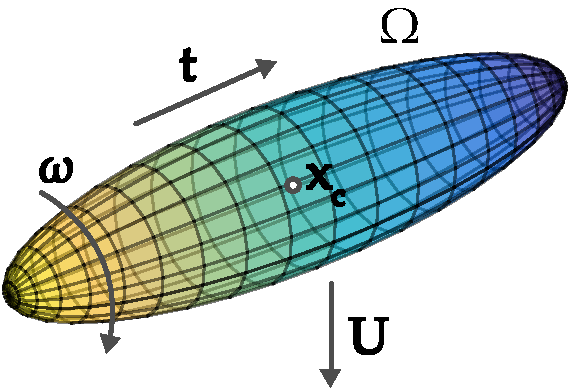
\includegraphics[width=.8\textwidth]{img/immersed_rigid.png}
  \caption[Two immersed objects in stokes flow.]{Two immersed objects in stokes flow, using a rigid body motion. Each fiber is characterized by the positions $\POS^1, \POS^2$ and the orientations $\ORIENT^1,\ORIENT^2$. The velocity of each point the surfaces $\Gamma^1, \Gamma^2$ is given by the rigid body motion described in Eqn~\eqref{eq:rigid_body_motion}.}
  \label{fig:immersed_rigid}
\end{figure}

By combining rigid body motion, Eqn.~\eqref{eq:rigid_body_motion}, with a boundary integral formulation of the Stokes equations a relationship between the objects velocities and the force distribution, $f$, acting on the surface of the object is given by,
\begin{equation}
  \label{eq:objects_boundary}
	\mathbf{U}_i^m + (\mathbf{\omega}^m \times (\POS - \POS_c^m))_i = \frac{1}{8 \pi \mu} \sum_{l=1}^{M} \int_{\Gamma^l} S_{ij}(\mathbf{x},\mathbf{y})f_j^l(\mathbf{y}) \, dS_y \quad i,j =1,2,3 \text{.}
\end{equation}

For a sedimenting object, the translational and rotational velocities $\mathbf{U}^m$ and $\mathbf{\omega}^m$ as well as the force distribution $\mathbf{f}^m$ are unknown. In order to be able to solve the system we use the additional constraints
\begin{equation}
	\label{eq:objects_boundary_constraints}
	\mathbf{F}_{\text{object}}^m = \int_{\Gamma^m} \mathbf{f}^m(\mathbf{y}) \, dS_y\text{,} \quad \mathbf{T}_{\text{object}}^m = \int_{\Gamma^m} (\POS - \POS_c^m) \times \mathbf{f}^m(\mathbf{y}) \, dS_y \text{,}
\end{equation}
stating that the integrated force and torque over each object must be equal to the externally applied force and torque on the object. Given these additional constraints we are now able to solve Eqns.~\eqref{eq:objects_boundary} and~\eqref{eq:objects_boundary_constraints} for $\mathbf{f}^m$, $\mathbf{U}^m$ and $\mathbf{\omega}^m$ for all fibers $m=1,2,\dots,M$. Once we have the velocities, $\mathbf{U}^m$ and $\mathbf{\omega}^m$, we can update the position and orthonormal basis of each object by solving,
\begin{equation}
	\label{eq:objects_update}
	\frac{d}{dt}\POS_c^m = \mathbf{U}^m \text{,} \quad \frac{d}{dt}\ORIENT^m = \ORIENT^m \times \mathbf{\omega}^m \text{.}
\end{equation}
The integral appearing in the right-hand side of Eqn.~\eqref{eq:objects_boundary} must in most cases be evaluated by numerical quadrature.

\section{Slender fibers}
\label{sec:slender_fibers}

The formulation developed in the previous section will now be adapted for a rigid fiber suspension. Consider a straight, rigid body of length $2L$ and radius $a$, and let $\epsilon = a / 2 L$ denote a slenderness parameter. If $\epsilon \ll 1$ the body is referred to as a slender body (slender fiber) as illustrated in Fig.~\ref{fig:slenderness}.

\begin{figure}[htbp]
  \centering
  \begin{subfigure}[h]{0.24\textwidth}
    \centering
    \includegraphics[width=\textwidth]{img/slender/1_4.png}
    \caption{$\epsilon=1/4$}\label{fig:slenderness_1_4}
  \end{subfigure}
  \begin{subfigure}[h]{0.24\textwidth}
    \centering
    \includegraphics[width=\textwidth]{img/slender/1_10.png}
    \caption{$\epsilon=1/10$}\label{fig:slenderness_1_10}
  \end{subfigure}
  \begin{subfigure}[h]{0.24\textwidth}
    \centering
    \includegraphics[width=\textwidth]{img/slender/1_20.png}
    \caption{$\epsilon=1/20$}\label{fig:slenderness_1_20}
  \end{subfigure}
  \begin{subfigure}[h]{0.24\textwidth}
    \centering
    \includegraphics[width=\textwidth]{img/slender/1_100.png}
    \caption{$\epsilon=1/100$}\label{fig:slenderness_1_100}
  \end{subfigure}
  \caption[Illustration of the slenderness parameters.]{Illustration of the slenderness parameters. When $\epsilon$ becomes smaller the shape of the body asymptotically approaches that of an infinitesimal slender fiber.}
  \label{fig:slenderness}
\end{figure}

Our goal is to simulate many slender fibers. However, using the 2D boundary integral formulation will be very expensive to solve numerically. As the aspect ratio $1/\epsilon$ of the fiber increases, the number of quadrature points must increase in order to accurately resolve the flow field around the fibers. However, for slender bodies a slender body approximation can be used instead. 

The slender body approximation is derived from the boundary integral formulation of the Stokes Eqns.~\eqref{eq:objects_boundary}. Using asymptotic analysis the governing surface integrals are reduced to 1D integral equations along a centerline of the fiber. By matching the fluid velocity at a virtual boundary of a slender ellipsoid to the fiber centerline velocity, see Götz,~\cite{Gotz2000}. The accuracy of this approximation is in $O(\epsilon).$ The reduction in dimensionality from 2D boundary integral equations to 1D integral equations is crucial for the ability to include a large number of fibers in the simulations.

The slender body approximation yields a coupled system of 1D integral equations over two fundamental solutions of the Stokes equations, the Stokeslet, Eqn.~\eqref{eq:stokeslet_stokeslet} and the Doublet, Eqn.~\eqref{eq:doublet}. The coupled system relates the forces exerted on the fibers to their velocities and captures the non-local interaction of the fiber with itself (as mediated by the fluid), as well as with any other structures with the fluid, such as other fibers or external boundaries. The system of integral equations is solved using a boundary integral method. Details of the model are given in Tornberg and Gustavsson,~\cite{Tornberg2006}.

\begin{figure}[htbp]
  \centering
  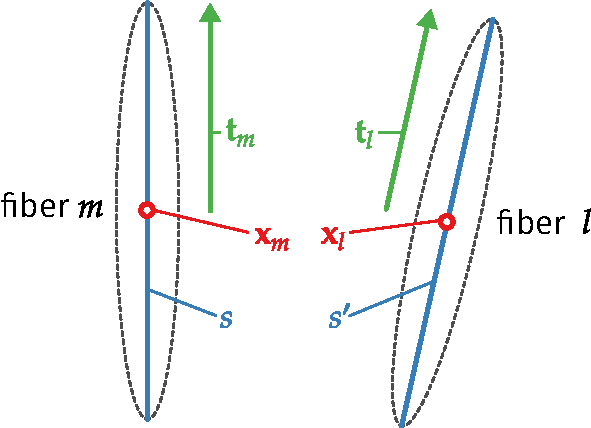
\includegraphics[width=0.5\textwidth]{img/slender.pdf}
  \caption[Slender fiber approximation.]{Slender fiber approximation. Each fiber is described by the center points $\POS_m, \POS_l$ the orientations given by the unit tangent vectors $\ORIENT_m, \ORIENT_l$ and the center line parameterized by $s$ and $s'$. The points on each center line is thus given by $\POS_m(s) = \POS_m + s\ORIENT_m$.}
  \label{fig:slender_fiber}
\end{figure}

Assume that we have $M$ fibers immersed in the fluid. As shown in Fig.~\ref{fig:slender_fiber} each fiber is now defined by its centerline and parameterized by the arc-length, ${s \in [-L,L]}$. For fiber $m$ the coordinates of the centerline are given by \linebreak[4]${\POS_m(s,t) = \POS_m(t) + s\ORIENT_m(t)}$, where $\POS_m$ is the center point and $\ORIENT_m$ the unit tangent vector of the fiber and ${m=1,2,\dots,M}$.

If the fluid exerts a force per unit length, $\mathbf{f}_m$ on fiber $m$, the slender body approximation for the velocity of the centerline of fiber $m$ can be stated in non-dimensional form as
\begin{equation}
  \label{eq:velocity_centerline}
  \begin{aligned}
    d(\dot{\POS}_m + s \dot{\ORIENT}_m) &= \left[ d(\mathbf{I} + \ORIENT_m\ORIENT_m^\top) + 2(\mathbf{I} - \ORIENT_m\ORIENT_m^\top)\right]\mathbf{f}_m(s) \\
    &+ (\mathbf{I} + \ORIENT_m\ORIENT_m^\top)\bar{\mathbf{K}}[\mathbf{f}_m](s) + \mathbf{V}_m(s) \text{.}
  \end{aligned}
\end{equation}
Here $d$ is a geometry parameter,
\begin{equation}
  \label{eq:geometry_parameter}
  d = -\ln{\epsilon^2e} \text{,}
\end{equation}
and $\bar{\mathbf{K}}[\mathbf{f}_m](s)$ is an integral operator given by
\begin{equation}
  \label{eq:integral_operator}
  \bar{\mathbf{K}}[\mathbf{f}_m](s) = \int_{-1}^{1} \frac{\mathbf{f}(s') - \mathbf{f}(s)}{|s' - s|} \, ds' \text{.}
\end{equation}

The contribution to the velocity of fiber $m$ from the other fibers in the system is accounted for in $\mathbf{V}_m(s)$ as
\begin{equation}
  \label{eq:velocity_contribution}
  \mathbf{V}_m(s) = \sum_{\substack{l=1\\l \neq m}}^M \int_{-1}^{1} \mathbf{G}(\mathbf{R}_{lm}(s,s'))\mathbf{f}_l(s') \, ds' \text{,}
\end{equation}
where $\mathbf{R}_{lm}(s,s') = \POS_m + s\ORIENT_m - (\POS_l + s'\ORIENT_l)$ is the distance between one point on fiber $m$ and one point on fiber $l$ as illustrated in Fig.~\ref{fig:fiber_contribution}.

\begin{figure}[htbp]
  \centering
  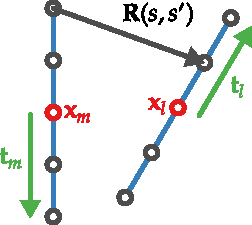
\includegraphics[width=0.3\textwidth]{img/fiber_contribution.pdf}
  \caption[Two interacting fibers with five quadrature points.]{Two fibers with five quadrature points each. The interaction between two fibers is given by the term $\mathbf{V}_m$ and depends solely on the distance between the two. The integral in Eqn.~\eqref{eq:velocity_contribution} can not be evaluated analytically and will be approximated by a quadrature rule.}
  \label{fig:fiber_contribution}
\end{figure}

The Green's function in this case is a linear combination of two fundamental solutions and reads
\begin{equation}
  \label{eq:green_function}
  \mathbf{G}(\mathbf{R}) = \begin{dcases*}
  \mathbf{S}(\mathbf{R}) + 2\epsilon^2\mathbf{D}(\mathbf{R}) & if $l \neq m$\\
  0 & if $l = m$
  \end{dcases*}
\end{equation}
with $\mathbf{S}$ and $\mathbf{D}$ as defined in Eqns.~\eqref{eq:stokeslet_stokeslet} and~\eqref{eq:doublet}.

In the non-dimensionalization the half-length of the fiber has been used as a characteristic length, $L_c = L$. This will give us a characteristic velocity and time as
\begin{equation}
  U_C = \frac{d \Delta \rho g V}{4\pi\mu_fL} \text{,} \quad T_C = \frac{2\pi\mu_fL^2}{d \Delta \rho g V} \text{.}
\end{equation}

The unknowns in Eqns.~\eqref{eq:velocity_centerline} are the translational and rotational velocities, $\dot{\POS}_m$ and $\dot{\ORIENT}_m$ and the force distribution along the fiber $\mathbf{f}_m(s)$. To close the formulation we use the additional conditions stating that the integrated force and torque on each fiber must balance the external forces and torques applied to the fibers,
\begin{equation}
	\label{eq:slender_boundary_constraints}
  \mathbf{F}_m = \int_{-1}^{1} \mathbf{f}_m(s) \, ds = \mathbf{F}_g \text{,} \quad \mathbf{T}_m = \int_{-1}^{1} s(\ORIENT_m \times \mathbf{f}_m(s)) \, ds = 0 \text{.}
\end{equation}
For our simulation the external force is just gravity and the external torque is set to zero. 

\chapter{Numerical algorithm and serial implementation}
\label{cha:serial_implementation}

In the last chapter, we presented the theoretical foundation of the physics and mathematics involved in simulating rigid fibers. Based on the Stokes Equation, we introduced the framework of boundary integral methods to efficiently model the behavior of rigid fibers. Using this background we will now review the numerical approach used for the simulation.

We will separate the overall algorithm into four steps and discuss each step individually. Additionally, we will touch upon implementation details used in the original serial version. We close the chapter with a brief reflection of the performance characteristics of the serial implementation to guide the parallel implementation on the GPU.

\section{Assemble System}
In the previous chapter we obtained the final closed system and the equations~\eqref{eq:velocity_centerline}~and~\eqref{eq:slender_boundary_constraints}. By integrating equation~\eqref{eq:velocity_centerline} from $-1$ to $1$ we can derive two separate equations for $\mathbf{\dot{x}}_m$ and $\mathbf{\dot{t}_m}$. Using these two equations and some algebra we can obtain a system of equations for $\mathbf{f}_m$ for all fibers from $m=1,2,\dots,M$, which only include computable quantities. For more details and an in depth discussion please refer to the original paper by Tornberg and Gustavsson~\cite{Tornberg2006}.

In order to be able to solve these equations for $\mathbf{f}_m$ we have to discretize them. For this we expand the force as a sum of $N+1$ Legendre polynomials $P_n(s)$
\begin{equation}
  \label{eq:force_discretization}
  \mathbf{f}_m = \frac{1}{2}\mathbf{F}_g + \sum_{n=1}^{N}a_{m}^{n} P_n(s) \text{,}
\end{equation}
where the coefficients $a_{m}^{n}$ are vectors with three components. The number of Legendre polynomials $N$ used for the force expansion is a parameter and is set to $5$ in our simulation.

\subsection{Closed linear system}

Using the force expansion from equation~\ref{eq:force_discretization} in equation~\ref{eq:slender_fibers_velocity} we get a closed linear system of equations for the coefficients $a_{m}^{n}$ for $n=1,\dots,N$ force expansions and $m = 1,\dots,M$ fibers.

For a 3-dimensional simulation, this results in a linear system of size $3MN\times3MN$. The first step of the algorithm is thus to compute and assemble the linear system in memory. Writing the system in the standard form $\mathbf{A}\mathbf{\bar{a}}=\mathbf{b}$ gives the following structure for the matrix $A$ and the right-hand side $b$
\begin{equation}
  \label{eq:matrix_structure}
  \renewcommand\arraystretch{1.5}
  \mathbf{A} =
  \begin{bmatrix}
    \mathbf{I} & \bar{A}_{12} & \cdots & \bar{A}_{1M} \\
    \bar{A}_{21} & \mathbf{I} & \cdots & \bar{A}_{2M} \\
    \vdots & \vdots & \ddots & \vdots \\
    \bar{A}_{M1} & \bar{A}_{M2} & \cdots & \mathbf{I}
  \end{bmatrix} \text{,} \quad \mathbf{b} =
  \begin{bmatrix}
    \bar{b}_{1} \\
    \bar{b}_{2} \\
    \vdots \\
    \bar{b}_{M} \\
  \end{bmatrix} \text{.}
\end{equation}
In this notation $\bar{A}_{ml}$ describes the $3N\times3N$ matrix encapsulating the contribution from the force coefficients on fiber $l$ onto the force coefficients for fiber $m$.

\subsection{Inner integral}
\label{subsec:inner_integral}

For each $\bar{A}_{ml}$, a $3\times3$ matrix, $\Theta_{lm}^{kn}$, where
\begin{equation}
  \label{eq:inner_integral}
  \Theta_{lm}^{kn} = \int_{-1}^{1} \left[\int_{-1}^{1}\mathbf{G}(\mathbf{R}(s,s')) P_k(s') \, ds' \right]P_n(s) \, ds \text{,}
\end{equation}
has to be evaluated for each force index $k,n = 1,2,\dots,N$. $G$ and $R$ are defined as in equation~\eqref{eq:G}~and~\eqref{eq:fiber_distance}, respectively. This can be achieved by using a standard Gaussian quadrature approach for both the inner and outer integral. However, as fibers get very close the number of quadrature points have to increase to accurately compute the fiber interactions. Unfortunately, doing so also increases the unknowns in the system, which in turn decreases the performance. For our simulation we use the same approach as the original paper. We divide each fiber into 8 subintervals and use a three-point gaussian quadrature on each interval. This results in a total of $3 \times 8 = 24$ quadrature points per fiber, which represents a good trade-off between accuracy and performance.

Another option is to find an analytical solution for the inner integral and only solve the outer integral numerically. We will not discuss the detailed derivation of the analytical solution, for an in-depth discussion please see~\cite{Tornberg2006}. In theory this approach allows for perfect accuracy for the inner integral, however in practice this is limited by the numerical precision of the simulation. The obtained formulas are recursive and thus sensitive to round off errors. To minimize the accumulation of round off errors, the original serial implementation uses a trick and switches the direction of the recursion, depending on how far apart the fibers are. This improves the practical accuracy and did not have a negative effect on performance.

Choosing between both options requires a careful examination of the accuracy and performance trade-off and is depend on the simulation setup. For the original serial implementation the combined numerical and analytical approach for evaluation proved to be the fastest and was thus chosen as the default. We will later explore how is applies to the new parallel GPU implementation.

\section{Solve System}

After having assembled the linear system $\mathbf{A}\mathbf{\bar{a}}=\mathbf{b}$ the next step to solve it. This can be done using standard linear equation solvers. This step is treated as a black box by the simulation, simply plugging in the matrix $\mathbf{A}$ and the vector $\mathbf{b}$ and getting back the solution vector $\mathbf{\bar{a}}$ representing the force coefficients.

The linear system can either be solved using a direct solver or an iterative method like GMRES. Unfortunately the matrix is neither symmetric nor sparse so we can't take advantage of specialized solvers for these cases~\cite{Tornberg2006}. As long as the fibers are sufficiently far apart and the matrix is not ill-conditioned, GMRES is able to solve the system in less than $10$ iterations. This is the reason why the original serial implementation uses GMRES by default. How the different solvers perform on the GPU will be compared in section~\ref{sec:bench_linear_solvers}.

\section{Update Velocities}

The force coefficients obtained by solving the linear system can now be used to calculate the remaining unknowns. By using the force expansion in the two separate equations for $\mathbf{\dot{x}}_m$ and $\mathbf{\dot{t}_m}$. The required implementation is thus similar to the computations for the \emph{Assemble System} step. The two integrals, again, can be evaluated either exclusively numerical or with the combined approach of solving the inner integral analytically.

\section{Update Fibers}
\label{sec:serial_update_fibers}

The final step takes care of advancing the fibers forward in time. The equations do not impose any strict stability restrictions, so an explicit time-stepping scheme can be used. We also use the same second order multi-step method used in the original paper. The update for the position of the center coordinate $\mathbf{x}_m$ is given by the following discretization in time
\begin{equation}
  \label{eq:time_discretization}
  \frac{3\mathbf{x}_m^{i+1} - 4\mathbf{x}_m^{i} + \mathbf{x}_m^{i-1}}{2 \Delta t} = (2\mathbf{\dot{x}}_m^{i} - \mathbf{\dot{x}}_m^{i-1}) \text{,}
\end{equation}
where the time step is denoted by $\Delta t$ and superscripts denote the numerical approximation of $\mathbf{x}_m(t_i)$. In order to compute the next state this method requires both the previous and the current state. As there is no previous time step for $t_0$, the first step $\mathbf{x}_{m}^{1}$ is computed by a simply first order forward Euler method. The calculation for the orientation vector $\mathbf{t}_m$ is computed using the same discretization by replacing the translational velocity $\mathbf{\dot{x}}_m$ with the rotational velocity $\mathbf{\dot{t}}_m$. Additionally, we must renormalize the orientation vector so that it maintains its unit length.

At the end of this step the state of the fibers can optionally be written to an external file for post processing and visualization in other tools. After completing this step, the algorithm starts again from the top with the \emph{Assemble System} step. This cycle repeats until a specified number of time steps have been executed.

\section{Algorithm summary}
\label{sec:algorithm_summary}

The original paper implemented this algorithm using Fortran. The computation were all performed in double precision and executed using a single thread on the CPU. In summary the four steps of the algorithm are at each timestep $t=t^n$ given the fiber configuration in terms of position, $x_m$, and orientation, $t_m$, 
\begin{description}
  \item[1. Assemble System] Computes all interactions between fibers and yields linear system $\mathbf{A}\mathbf{\bar{a}}=\mathbf{b}$
  \item[2. Solve System] 
  \item[3. Update Velocities] Computes velocities $\mathbf{\dot{x}}$ and $\mathbf{\dot{t}}$
  \item[4. Update Fibers] Yields new fiber configuration at $t=t^{n+1}$
\end{description}

Empirical results show that the majority of the required computation time is spent on the 1.~\emph{Assemble System} and 3.~\emph{Update Velocities} steps. The time required for advancing the simulation state in step 4.~\emph{Update Fibers} is completely negligible. We will see later in Chapter~\ref{cha:benchmarks} that the same holds true for the new parallel implementation.

Since we won't be writing our own implementation of linear solvers on the GPU we have only limited influence on the performance of the 2.~\emph{Solve System} step. We instead treat it as a black box and rely on the efficiency of pre-existing libraries. The only control we have is the choice which library and solver to use. For direct solvers the computation time only depends on the number of unknowns and is approximately constant throughout the simulation. The performance of iterative solvers on the other hand is highly depend on the condition number of the matrix and thus unpredictable. In line with the original paper we will both test a direct solver and iterative solvers to get a better understanding of their respective performance behavior.

Consequently, the most important step to optimize is 1.~\emph{Assemble System}. Fortunately it is well suited for parallelization. The fibers can be partitioned naturally across the compute units, where each unit is responsible for a subset of fibers. The focus of the optimization will thus lie on the \emph{Assemble System}. As the required computation for the 3.~\emph{Update Velocities} step is similar it will also indirectly benefit from any optimizations. Additionally, we will also look at how the two different options for solving the integral in equation~\ref{eq:inner_integral} perform in the parallel environment. Therefore, the next goal is to parallelize each algorithm step on the GPU.


\chapter{GPU Programming}
\label{cha:gpu_programming}

In the previous chapter the numerical algorithm and its serial implementation was presented. It discussed various implementation details which have to be considered to arrive at the most efficient implementation.

To further increase the efficiency modern GPUs offer a massively parallel architecture to accelerate many different applications. We will begin with a short introduction to general purpose computing on GPUs. Afterwards, different Application Programming Interfaces (API) for programming on GPUs are discussed regarding their advantages and disadvantages. The chosen API, CUDA, will be presented with its programming model at the end of this chapter.

\section{General Purpose Computing on GPUs}
In the beginning Graphics Processing Units were highly specialized pieces of hardware developed to exclusively improve the performance of real-time 3D graphics. However, in recent years GPUs have started to be used for running arbitrary code instead of being limited to graphics related computations. This allows for impressive performance increases across a wide range of different general purpose applications. A good overview of the evolution of GPU computing can be found in Owens et al.~\cite{Owens2008}.

The deciding factor for the performance is how well the application can be parallelized to take advantage of the massively parallel architecture of GPUs. This massive parallelism has lead to potentially large performance advantages of GPUs over CPUs as illustrated in Fig.~\ref{fig:gpu_performance}. It shows the year over year increase in the theoretical floating point operations per second (FLOP/s). The FLOP/s number is calculated by combining information of the number of compute units, frequency and memory bandwidth for both the CPU and GPU models. This does not necessarily translate to direct real world performance increases but tries to visualize the potential GPUs have.

\begin{figure}[!htbp]
  \centering
  \begin{tikzpicture}
    \begin{axis}[
      title=Theoretical GFLOP/s,
      xlabel={Year},
      ylabel={GFLOP/s},
      date coordinates in=x,
      xticklabel={\year},
      date ZERO=2002-01-01,
      xtick={2002-01-01,2004-01-01,2006-01-01,2008-01-01,2010-01-01,2012-01-01,2014-01-01},
      xmin=2002-01-01,
      xmax=2014-01-01,
      ymin=0,ymax=5500,
      ]
      \addplot[color=set12_light,mark=*,mark options={fill=white}, very thick] table[x=Date,y=Double,col sep=comma,meta=Name] {charts/cpu_performance.csv};
      \addlegendentry{Intel CPU Double Precision}

      \addplot[
      scatter,
      visualization depends on=\thisrow{alignment} \as \alignment,
      nodes near coords,
      point meta=explicit symbolic,
      every node near coord/.style={anchor=\alignment},
      color=set13_light,
      mark=*,
      mark options={fill=white},
      very thick,
      every node near coord/.append style={font=\tiny},
      ] table[x=Date,y=Double,col sep=comma,meta=Name] {charts/double_gpu_performance.csv};
      \addlegendentry{NVIDIA GPU Double Precision}

      \addplot[
      scatter,
      visualization depends on=\thisrow{alignment} \as \alignment,
      nodes near coords,
      point meta=explicit symbolic,
      every node near coord/.style={anchor=\alignment},
      color=set12,
      mark=*,
      mark options={fill=white},
      very thick,
      every node near coord/.append style={font=\tiny},
      ] table[x=Date,y=Single,col sep=comma,meta=Name] {charts/cpu_performance.csv};
      \addlegendentry{Intel CPU Single Precision}
      \addplot[
      scatter,
      visualization depends on=\thisrow{alignment} \as \alignment,
      nodes near coords,
      point meta=explicit symbolic,
      every node near coord/.style={anchor=\alignment},
      color=set13,
      mark=*,
      mark options={fill=white},
      very thick,
      every node near coord/.append style={font=\tiny},
      ] table[x=Date,y=Single,col sep=comma,meta=Name] {charts/single_gpu_performance.csv};
      \addlegendentry{NVIDIA GPU Single Precision}

    \end{axis}
  \end{tikzpicture}
  \caption[Year over year increase in theoretical floating-point operations per second for CPUs and GPUs.]{Year over year increase in theoretical floating-point operations per second for CPUs and GPUs~\cite{CudaProgrammingGuide}.}
  \label{fig:gpu_performance}
\end{figure}

The huge difference in performance between a GPU and a CPU mainly derives from the number of independent compute units. How a compute unit is exactly defined differs between architectures and vendors. On a CPU the number of compute units usually refers to the number of CPU cores. Each individual CPU cores is very fast, however, CPUs usually only have four, eight or maybe sixteen cores. In contrast to this, GPUs can have several hundreds of independent compute units. Each GPU compute unit can perform calculations in parallel and thus provides the opportunity to yield big performance improvements for high-throughput type computations. This is one reason why g general purpose computing on GPUs was introduced to the world of supercomputers. Over time, a growing number of supercomputers started supplementing their computing power with GPUs and some even rely exclusively on GPUs for their computations.

In order to take advantage of these new massively parallel architectures new API had to be developed. The two proposed APIs are OpenCL and CUDA. OpenCL is an open and cross platform standard maintained by the Khronos Group~\cite{OpenCL}. The same group is also responsible for its graphics focused counterpart OpenGL. OpenCL is not exclusive to GPUs, but instead tries to be a general abstract layer for different parallel architectures. This allows OpenCL code to be run not only on GPUs but also on CPUs. CUDA on the other hand is developed by NVIDIA exclusively for their line of GPUs.

\section{CUDA vs. OpenCL}

Choosing between OpenCL and CUDA is the first decision to be made when starting to implement a new project on GPUs. The main advantage of OpenCL is the ability to run on many different devices. All major players in the computing space provide an implementation on top of their platforms. Both Intel and AMD provide the API for their CPU and both AMD and NVIDIA have drivers available for their GPUs. However, this advantage can also be a disadvantage as the achievable performance might suffer from the abstraction across all platforms. The OpenCL framework is potentially not optimized for a particular device specific architecture. CUDA on the contrary is in theory highly optimized to achieve the best possible performance on NVIDIA's GPUs. In practice the difference can possibly be mitigated by spending the extra time to fine-tune the OpenCL implementation to the hardware's specific needs. Another disadvantage of OpenCL is the potentially outdated and inconsistent driver support for the various devices. This is especially true for NVIDIA who seem to have stopped updating OpenCL, still only supporting OpenCL 1.1 which was released back in 2010. Their main focus is on pushing CUDA and updating it to support all the feature in their new GPUs.

For this thesis we chose to go with NVIDIA's CUDA framework mainly because of the available hardware both at the workstation computers and at the local computing cluster. Additionally, this project does not need the cross-platform capability as the main focus is on pure performance in a highly specialized setup and simulation scenario. The application will not be widely distributed and only used for internal purposes.

\section{CUDA Programming Model}
\label{sec:CUDA}
The abbreviation CUDA stands for Compute Unified Device Architecture and was introduced by NVIDIA in 2006 as a general purpose parallel computing platform. It leverages the highly parallel architecture of modern NVIDIA GPUs to solve many different computational problems, which can lead to potentially large performance improvements compared to traditional CPUs.

The CUDA platform allows developers to use a variety of different options to program the GPU. The easiest way is to link to any CUDA-accelerated library and simply using the libraries interfaces from any software environment. For more advanced uses extensions to various programming languages exist like C/C++, Fortran and even managed languages like Java, Python and many more. This allows for easy and fast integration into any software environment the developer is comfortable with. Fig.~\ref{fig:cuda_overview} illustrated the different components of the overall CUDA platform.

\begin{figure}[!htbp]
  \centering
  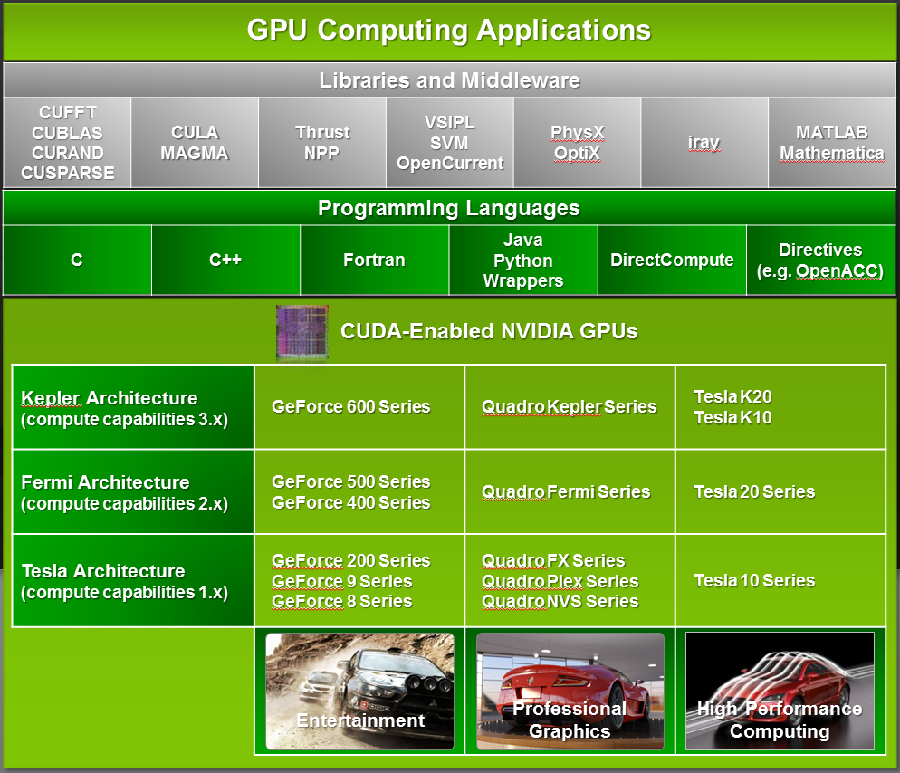
\includegraphics[width=.9\textwidth]{img/cuda_overview.pdf}
  \caption[Overview of the CUDA platform.]{Overview of the CUDA platform~\cite{CudaProgrammingGuide}.}
  \label{fig:cuda_overview}
\end{figure}

The basic building blocks of the CUDA Programming Model from a development perspective are kernels. CUDA kernels are the equivalent of normal C functions. However, the major difference is that instead of being executed just once, kernels are executed in parallel by $N$ different threads. These CUDA threads are distributed and run across the available compute units of the GPU. To illustrate how a very basic kernel invocation looks, Listing~\ref{lst:code_vector_addition} shows a code sample for a very simple vector addition.

\begin{listing}[!htbp]
  \centering
  \inputminted[mathescape,
    linenos,
    numbersep=5pt,
    fontsize=\footnotesize,
    frame=lines,
    framesep=2mm]{c}{lst/cuda_vector_add.lst}
  \caption{Pseudocode for CUDA vector addition.}
  \label{lst:code_vector_addition}
\end{listing}

\paragraph{CUDA Kernels}

It is important to remember that each kernel invocation is executed independently and no ordering is guaranteed. It is therefore essential to avoid any order-dependent operations or shared memory access. There are however, ways to allow for shared memory access which will be briefly touched upon later in the practical implementation of the simulation.

\paragraph{Thread Hierarchy}

In order to efficiently distribute the different threads across the compute units of the GPU, CUDA defines a thread hierarchy. As discussed previously a GPU consists of many independent compute units. On NVIDIA GPUs these units are referred to as Streaming Multiprocessors (SMs). During execution of the application each SM is tasked with running a distinct set of threads. In CUDA these sets of threads are called thread blocks. Each thread block is distributed to all the available SMs, which allows for automatic scalability depending on the number of SMs available  as illustrated in Fig.~\ref{fig:automatic_scaling}. Thus the developer only has to divide the workload into appropriately sized blocks of threads and invoke the kernel.

\begin{figure}[!htbp]
  \centering
  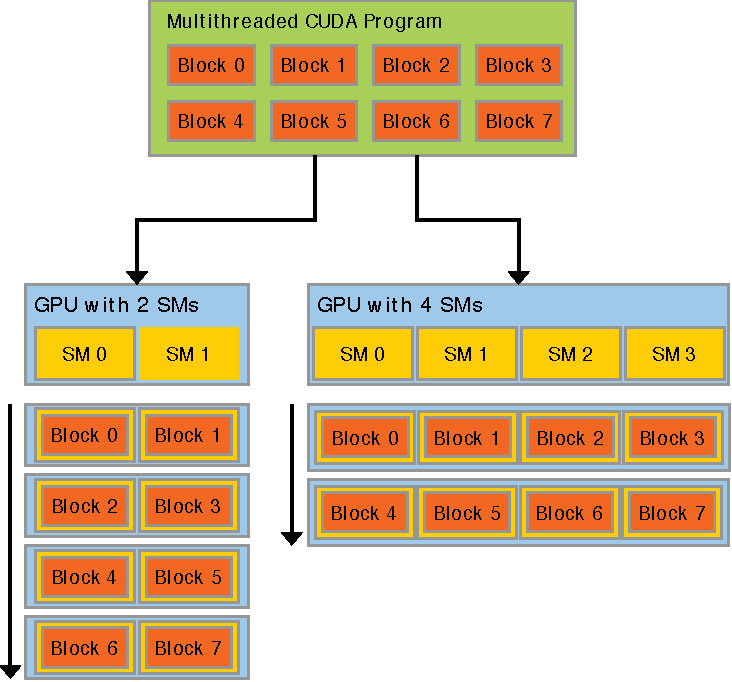
\includegraphics[width=\textwidth]{img/automatic_scaling.pdf}
  \caption[Automatic scaling of blocks across an arbitrary number of Streaming Multiprocessors.]{Automatic scaling of blocks across an arbitrary number of Streaming Multiprocessors~\cite{CudaProgrammingGuide}.}
  \label{fig:automatic_scaling}
\end{figure}

How to choose the optimal size of a block in order to maximize the performance is not an easy question to answer and it is highly dependent on the particular task and implementation. In practice the size is often chosen by running benchmarks with various sizes to determine the optimal configuration.

In order to make programming easier, CUDA blocks can be addressed using either a one-dimensional, two-dimensional, or three-dimensional thread index. For example in the case of a calculation involving matrices, it is more natural to think about parallelizing each element given by the row and column index instead of a single one-dimensional index. This is illustrated in the code sample in Listing~\ref{lst:code_matrix_addition}

\begin{listing}[!htbp]
  \centering
  \inputminted[mathescape,
    linenos,
    numbersep=5pt,
    fontsize=\footnotesize,
    frame=lines,
    framesep=2mm]{c}{lst/cuda_matrix_add.lst}
  \caption{Pseudocode for CUDA matrix addition, illustrating 2D thread blocks.}
  \label{lst:code_matrix_addition}
\end{listing}

Finally, as the resources of each Streaming Multiprocessor are limited, there is an upper bound of how many threads a block can contain. Currently this maximum number of threads is $1024$. This means that the maximum size of matrices, that can be added with the two-dimensional thread block code sample in Listing~\ref{lst:code_matrix_addition} is $32\times32 = 1024$. To solve this problem CUDA introduces another layer above blocks called a grid. A grid organizes thread blocks again into either one, two, or three dimensions. The number of thread blocks in a grid is unlimited and thus solely dependent on the size of the workload. Fig.~\ref{fig:grid_blocks} shows an example configuration of a 2D grid with 2D blocks.

\begin{figure}[!htbp]
  \centering
  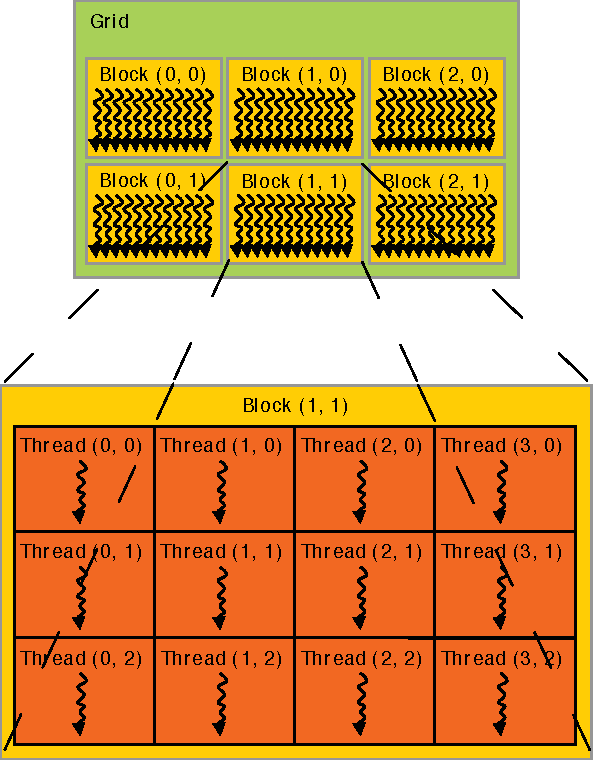
\includegraphics[width=0.6\textwidth]{img/grid_blocks.pdf}
  \caption[CUDA block addressing using 2D grid with 2D thread blocks.]{CUDA block addressing using 2D grid with 2D thread blocks~\cite{CudaProgrammingGuide}.}
  \label{fig:grid_blocks}
\end{figure}

\paragraph{Memory Hierarchy}

In addition to the \emph{Thread Hierarchy} CUDA also implements a 3 layer memory hierarchy as illustrated in Fig.~\ref{fig:memory_hierarchy}. Each level of this hierarchy differs in size, latency and scope. The sizes refers to amount of bytes that can be stored in the level and latency to the time it between requesting data and being able to actually use it. Additionally each level is confined to a specific scope, restricting from where the data can be accessed.

The first level contains the fastest and smallest memory. This is a private memory where each thread has its own area and only this thread can read from and write to this area. How much space each thread has is determined by how many threads are executed on each SM. The more memory an individual thread requires the fewer threads can run in parallel on a SM. Optimizing this trade-off is important for achieving a good performance. On the newest GPUs each SM has $65536 * 32\text{-bit} = 256\text{KB}$ to divide among the threads.

The second level is called shared memory, or sometimes local memory. Although it is slower than the private memory, it has the advantage that all threads executing on an SM have simultaneous access to it. This allows different threads to cooperate and share work. Depending on the characteristics of the algorithm, this can save a lot of computing time. Therefore it is important to analyze whether shared memory can actually improve the performance. The size of this memory level on current GPUs is around $64\text{KB}$ to $96\text{KB}$.

The third level contains the largest memory area which is called the global memory. This is the amount of memory used  on the packaging of the GPUs to advertise the product. Nowadays it is usually $2\text{GB}$ or $4\text{GB}$. It is accessible by all threads and stores all data relating to the current application. However, accessing it can be quite slow compared to the other levels of the memory hierarchy. Additionally, one has to be careful to avoid memory conflicts when accessing the same memory location form different threads at the same time. This is especially important since this can further reduce the performance. Taking everything into account, it can be said that it is an important optimization step to make access to global memory as efficient as possible. This can be achieved by intelligently packing data, or caching data in a lower level of the hierarchy. 

Another option to avoid the slow the performance of the global memory is to make sure that the required data for each individual thread from global memory is small enough. The associated latency when reading data from global memory can be hidden when enough calculation are performed on this data. The GPU is then able to quickly switch to another set of threads and continue the computation while waiting on data from global memory.

\begin{figure}[!htbp]
  \centering
  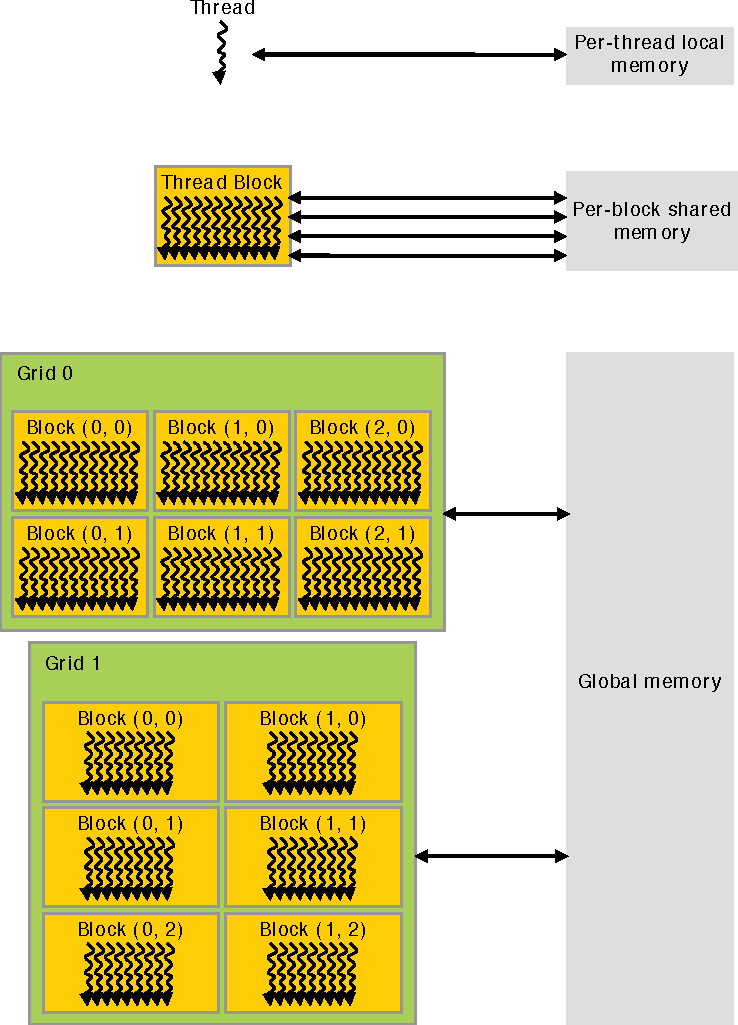
\includegraphics[width=0.8\textwidth]{img/memory_hierarchy.pdf}
  \caption[CUDA memory hierarchy.]{CUDA memory hierarchy~\cite{CudaProgrammingGuide}.}
  \label{fig:memory_hierarchy}
\end{figure}


\chapter{Parallel implementation}
\label{cha:parallel_implementation}

Based on the previous two chapters describing the serial Fortran implementation and GPU programming we will now look at the algorithm in more detail and show, how it is adapted to take advantage of multi-core architectures. The main focus of this thesis is the implementation of the algorithm on a modern massively parallel NVIDIA GPUs using CUDA. In order to gain a better understanding of the achievable performance improvements we additionally back-ported the finished GPU code of the algorithm to multi-core CPUs using the OpenMP framework.

We will begin by introducing the software tools and libraries utilized. Afterwards, we will explain the practical implementation of the algorithm in CUDA. This is followed by a discussion of several potential optimization approaches to further improve the performance of the implementation. The chapter ends with a brief explanation of OpenMP and how the code was parallelized on the CPU.

\section{Development environment}
The rigid fiber simulation algorithm developed as part of this thesis is only loosely based on the original serial Fortran implementation. The reason for this is to ensure a clean starting point and to avoid difficulties in adapting the existing code for parallel execution, as it was never intended to be run across multiple cores. This also provides an opportunity to learn from the shortcomings of the old code, and not only parallelize it but also improve the efficiency in general.

The development is done exclusively on a Linux workstation running Ubuntu as this will also be the exact same runtime environment used in later experiments. The build system for compiling and linking the final application is CMake,~\cite{CMake}. It is chosen because it is a widely used open-source and cross-platform build system, which allows for easy integration of the various required libraries in a well documented and straightforward manner. Under the hood the build system uses NVIDIA's CUDA platform tools to compile the code. For this NVIDIA includes the CUDA compiler, called \emph{nvcc}, capable of compiling C/C++ code together with the CUDA specific extensions.

In order to facilitate easier usage of the application both during development and later real-world usage a Python wrapper script is also available. The script completely automates the building process and dynamically customizes the application code to support three different modes of operation. The first is a simple \emph{run} mode which takes the supplied parameters and executes the simulation. The second mode is \emph{validate}, which allows for a fully automated way to test and validate different algorithm versions against a known correct simulation run. The \emph{validate} mode automatically computes the error and makes debugging of changes easier. The last mode is \emph{benchmark} which executes a particular simulation multiple times and collects and aggregates the timings for each simulation step as well as the total time.

\section{Linear solvers}
In addition to the CUDA platform, the application also requires support libraries for different linear solvers. During a simulation, a linear system of equations in the form of Eqn.~\eqref{eq:matrix_structure} has to be solved in each timestep. This can be one of the most time consuming parts of the algorithm. Hence, the overall simulation time relies heavily on the ability to solve large and dense systems as fast as possible. Therefore it is very important to weight all the available options carefully when choosing a particular linear solver algorithm or library.

In this work we have compared the performance of a direct solver to certain iterative solvers for solving the system. For the direct solver, the MAGMA library,~\cite{MagmaDocumentation}, is used and for the iterative we use the ViennaCL library,~\cite{ViennaCLDocumentation}. Both libraries will be introduced below.

\paragraph{MAGMA / CuBLAS / OpenBLAS}
MAGMA is a dense linear algebra library that provides features similar to standard LAPACK functions but for multicore architectures. It also has features to support hybrid algorithms for executing code across multiple GPUs or CPUs at the same time. However, these features are not explored in this thesis. Instead the focus is on a high performance single GPU implementation of a direct linear system solver.

MAGMA provides access to various high-level algebra routines, but the underlying math functions utilize the platform specific implementations of the BLAS levels. For CUDA this is implemented directly by NVIDIA in the form of the CuBLAS libraries,~\cite{CuBLAS}. Additionally, MAGMA tries to further improve their performance by combining GPU with CPU based algorithms. Thus a CPU based BLAS implementation is also needed. For this the OpenBLAS library,~\cite{OpenBLAS}, is chosen which is the most up-to-date and high performance library available apart from Intel's Math Kernel Library,~\cite{IntelMKL}. OpenBLAS takes full advantage of multicore systems and is also used for the comparison of our Fortran CPU implementation against the CUDA GPU implementation.

\paragraph{ViennaCL}
ViennaCL is an open-source linear algebra library developed at the University of Vienna. The library provides an abstraction layer across many different parallelization methods in order to facilitate consistent and easy to use support for BLAS level 1-3 and iterative solvers. This unique feature allows the developer to easily switch between different APIs and architectures for parallelization. Currently, the library supports OpenMP, OpenCL and most importantly for this thesis - CUDA.

ViennaCL's focus is on solving sparse matrices with the implemented iterative solvers. However, it also has basic support for solving dense matrices using a variety of different iterative solvers. As the rigid fiber simulation exclusively relies on dense matrices this makes it an ideal candidate for benchmarking. For this thesis the BiCGStab as well as the GMRES iterative solvers are used and tested.

\section{Kernels}
\label{sec:kernels}

The overall parallel algorithm is very similar to the serial version, however, each simulation step is separated into different kernels. Each kernel is invoked in a serial manner, this means that CUDA guarantees that all data modified in a kernel is available before the next kernel is executed. These kernels are then distributed across the GPU. All calculations are done using single precision floating point numbers, as NVIDIA limits high performance double precision computation to their server class GPUs. The CUDA pseudocode for the algorithm is illustrated in Listing~\ref{lst:pseudo_parallel_algorithm}. It begins by parsing the simulation parameters and the initial fiber configuration. After that, the required memory is allocated on the GPU. Finally, a simple loop executes all time steps and the four main algorithm sub steps — 1. \emph{Assemble System}, 2. \emph{Solve System}, 3. \emph{Update Velocities} and 4. \emph{Update Fibers} — as described in Sec.~\ref{sec:algorithm_summary} are run on the GPU.

\begin{listing}[htbp]
  \centering
  \inputminted[mathescape,
    linenos,
    numbersep=5pt,
    fontsize=\footnotesize,
    frame=lines,
    framesep=2mm]{c}{lst/parallel_algorithm.lst}
  \caption{Pseudocode for parallel algorithm on the host.}
  \label{lst:pseudo_parallel_algorithm}
\end{listing}

The application requires two general configuration files as an input. The first file is referred to as the parameters file which contains the different configuration variables and constants used throughout the algorithm. These include, for example the number and size of the time steps as well as the number of force expansion terms and quadrature points. Additionally, this file is also used to configure the iterative solvers like specifying the number of restarts for GMRES or the solution tolerance for BiCGStab and GMRES.

Each of the parallelized sub steps are now discussed in more detail. The purpose of each kernel as well as the required input and output are described below.

\paragraph{Assemble System}

\begin{listing}[htbp]
  \centering
  \inputminted[mathescape,
    linenos,
    numbersep=5pt,
    fontsize=\footnotesize,
    frame=lines,
    framesep=2mm]{c}{lst/assemble_system.lst}
  \caption{Pseudocode for the assemble system step with a 1D thread block.}
  \label{lst:pseudo_assemble_system}
\end{listing}

The \emph{Assemble System} kernel is the most important step of the algorithm, as it is the most time consuming step. This was already discussed in Sec.~\ref{sec:algorithm_summary} and it will also be shown in the benchmark tests presented in Chapter~\ref{cha:benchmarks}. 

The goal of the assembly step is to build the matrix and right-hand side for the linear system of equations in the memory. As an example Listing~\ref{lst:pseudo_assemble_system} shows a pseudocode for the \emph{Assemble System} step. In this example the code is parallelized using a one-dimensional thread block as described in Sec.~\ref{sec:CUDA}. This means that the code is parallelized for each fiber and that each thread calculates the contributions to this fiber from all the other fibers. Looking at the matrix in Eqn.~\eqref{eq:matrix_structure} each thread is thus responsible for $3*N$ rows of the matrix, where $N$ is the total number of terms in the force expansion in Eqn.~\eqref{eq:force_discretization}. Alongside the one-dimensional thread implementation other options exist. They will be discussed in the optimization Sec.~\ref{sec:parallel_optimizations}.

The kernel requires two inputs, the current position of each fiber and its orientation. Using these combined with the equations outlined in Chapter~\ref{cha:theoretical_foundation} and Chapter~\ref{cha:serial_implementation} the matrix and right-hand side elements are computed and used in the next step to solve the linear system they define.

\paragraph{Solve System}
As this thesis does not aim to implement generic linear solvers, this step is treated as a black box. In the \emph{Assemble System} kernel two arrays containing the matrix and right-hand side of the linear system have been computed. These two arrays are now passed to the library that implements the linear solver. In case of the direct solver it is the MAGMA library and for the two tested iterative solvers, BiCGStab and GMRES, it is the ViennaCL library. Both libraries are able to directly use the already allocated memory regions and no additional allocations have to be performed. In order to conserve memory space the resulting solution vector is stored in the same memory location as the right-hand side and is passed on to the subsequent steps.

\paragraph{Update Velocities}

\begin{listing}[htbp]
  \centering
  \inputminted[mathescape,
    linenos,
    numbersep=5pt,
    fontsize=\footnotesize,
    frame=lines,
    framesep=2mm]{c}{lst/update_velocities.lst}
  \caption{Pseudocode for the updating velocities simulation step.}
  \label{lst:pseudo_update_velocities}
\end{listing}

By solving the linear system of equations we obtain the coefficients in the force expansion as shown in Sec.~\ref{sec:serial_discretization}. The \emph{Update Velocities} kernel accumulates the exerted forces for all fibers and updates both the translational and the rotational velocities of the fibers simultaneously by computing the right-hand side in Eqns.~\eqref{eq:delta_translate_velocity} and~\eqref{eq:delta_rotate_velocity}. A two-dimensional thread block version of the kernel is illustrated in Listing~\ref{lst:pseudo_update_velocities}. In a two-dimensional thread block version each individual kernel invocation is responsible for a single pair of fiber interactions. In case of two different threads calculate the interactions for the same fiber, it might happen that they try to write their results to the same memory location. When this happens, it could lead to incorrect results for the velocities. Fortunately CUDA provides atomic functions to circumvent this issue which will be discussed in more detail in Sec.~\ref{subsec:bench_thread_block}. 

\paragraph{Update Fibers}

\begin{listing}[htbp]
  \centering
  \inputminted[mathescape,
    linenos,
    numbersep=5pt,
    fontsize=\footnotesize,
    frame=lines,
    framesep=2mm]{c}{lst/update_fibers.lst}
  \caption{Pseudocode for the updating fibers simulation step.}
  \label{lst:pseudo_update_fibers}
\end{listing}

The final simulation step takes care of advancing the position and orientation of the fibers in time. The pseudocode in Listing~\ref{lst:pseudo_update_fibers} implements the second-order multi-step method, Eqn.~\eqref{eq:time_discretization}, introduced in Sec.~\ref{sec:serial_update_fibers}. As it will be shown during benchmarking in Chapter~\ref{cha:benchmarks}, the required time for this kernel is minuscule compared to the other steps. The kernel scales linearly with the number of fibers and in addition it has a perfectly aligned memory access resulting in close to optimal usage of the GPU hardware.

\newpage
\section{Optimizations}
\label{sec:parallel_optimizations}

During the development of the parallel GPU implementation great care was taken to continuously optimize the code both on an algorithmic level as well as on an implementation level. Numerous small code-level optimizations have been performed based on the original serial code like precomputing as much data as possible, avoiding variable allocations or unnecessary copy operations in performance critical sections of the code.

Additionally, more advanced optimizations of the code were made like rearranging calculations inside loops to avoid executing redundant calculations and consolidating multiple loops into one. Finally, techniques such as loop unrolling and faster math functions, like the reciprocal of the square root, where also tested and included.

Throughout the optimization phase a benchmark suite was run after each step. This ensures that optimizations were only included if they had a measurable impact on the overall performance of the simulation. Moreover, with this approach potential performance regressions could be identified early and be avoided.

Many optimizations performed during this process are applicable to both the CPU and GPU implementations, since they showed performance improvements for both. However, some optimizations and algorithm variations are uniquely suited to the GPU hardware. Below we will look into three different optimizations on the GPU in more detail. The performance results for each will then later be discussed in Chapter~\ref{cha:benchmarks}.

\subsection{Numeric vs. analytic integration}
\label{subsec:numeric_analytic}
In the original paper,~\cite{Tornberg2006}, it was observed that the analytical integration of the inner integral in Eqn.~\eqref{eq:inner_integral} yielded a performance increase compared to purely numerical integration. Generally, using analytical integration should not only be preferred because of being faster but more importantly also because of being more accurate. However, for numerical precision reasons the actual implementation of the analytical integration can not achieve this theoretical level of accuracy. Especially for configurations with fibers that are very far apart the recursive implementation suffers from round-off errors and numerical instabilities. The steps taken to minimize these instabilities potentially affect the performance.

Based on these considerations and the fact that the computation of the integrals is a very performance critical part of the implementation, exploring the performance implications of both approaches on the GPU is of great interest. In contrast to the serial CPU implementation of the original paper, our implementation on the GPU is actually faster when solving both integrals numerically. We will discuss the reason and consequences of this in more detail in Sec.~\ref{subsec:bench_numeric_vs_analytic}.

\subsection{Shared memory}
\label{subsec:shared_memory}

As described in Sec.~\ref{sec:CUDA}, the CUDA code is subjected to a highly specialized memory hierarchy. Whereas traditional CPUs only have small caches and a large main memory pool, CUDA introduces the concept of a shared local memory space. The access time to this local memory is orders of magnitudes faster compared to accessing the global GPU memory. Additionally, local memory can be shared among the threads running on Streaming Multiprocessor and potentially save time by avoiding to constantly access the slow global memory. In order to test this, a shared memory version was implemented and tested for the \emph{Assemble System} step, since it is the most performance critical kernel.

To understand the idea, imagine the two-dimensional thread block implementation of the kernel. Then each thread block is responsible for many pairs of fiber interactions, e.g. fibers $[1,\dots,8]$ each interacting with fibers $[9,\dots,16]$. In total, these are $8 \times 8 = 64$ interactions. Each kernel invocation is responsible for one pair and has to load the position and orientation for the two interacting fibers. However, on closer inspection it is obvious that one does not need to load each fiber every time. As soon as fiber $1$ has been loaded into shared memory it can be reused for all the interactions with fibers $9$ through $16$ avoiding the unnecessary and slow access to global memory.

How this affects performance is not always easy to tell, as various factors can influence the result. One factor, for example, might be that the amount of necessary data is small enough to utilize memory caches and that repeated access to global memory can then automatically be avoided. Another factor is the performance characteristic of the kernel. Optimizing for shared memory usage only makes sense if on the one hand the kernel is memory bound, meaning that most of the execution time is spent waiting for data. If on the other hand, the kernel is compute bound the GPU is able to use time efficiently by performing pending computations while waiting for memory access. In this case forcing threads in a block to wait for shared data can actually decrease the overall performance of the kernel.

However, in general efficient exploitation of shared memory can be a huge advantage for parallel GPU implementations. This is especially true when comparing the performance to CPUs, as they do not have an equivalent fast and comparatively large memory space. Unfortunately, during our testing in Sec.~\ref{subsec:bench_shared_memory}, we did not see a performance advantage by using shared memory for the rigid fiber simulation.

\subsection{Thread block dimension}
\label{subsec:parallel_thread_block}

There are many different factors that determine the performance of a particular GPU algorithm. This is especially true with regard to optimally taking advantage of the specific underlying GPU architecture, which change even between different models of graphics cards. How to best utilize the hardware depends on specific memory access patterns, avoiding too much register usage and choosing optimal settings for the thread block size.

For this thesis we looked at the thread block dimension in particular and how choosing a different approach of parallelizing affects the performance. While doing so, the focus was on the \emph{Assemble System} step. However, the results were also transferred to the \emph{Update Velocities} step, which has a similar structure.

The kernel invocations for the one-dimensional and two-dimensional thread block approach are visualized in Fig.~\ref{fig:thread_block} using the matrix structure in Eqn.~\eqref{eq:matrix_structure} as an example. In the one-dimensional case each invocation is responsible for computing contributions to all sub matrices $\bar{A}_{ml}$. Thus in total this results in $M$ kernel invocations, one for each fiber. For the two-dimensional case each invocation is only responsible for the contribution to a single sub matrix. Here the total number of invocations is $M \times M$. The three-dimensional case divides the calculation for the sub matrix further, one additional invocation per force index for a total of $M \times M \times N$ invocations.

\begin{figure}[htbp]
  \centering
  \begin{subfigure}[h]{0.33\textwidth}
    \centering
    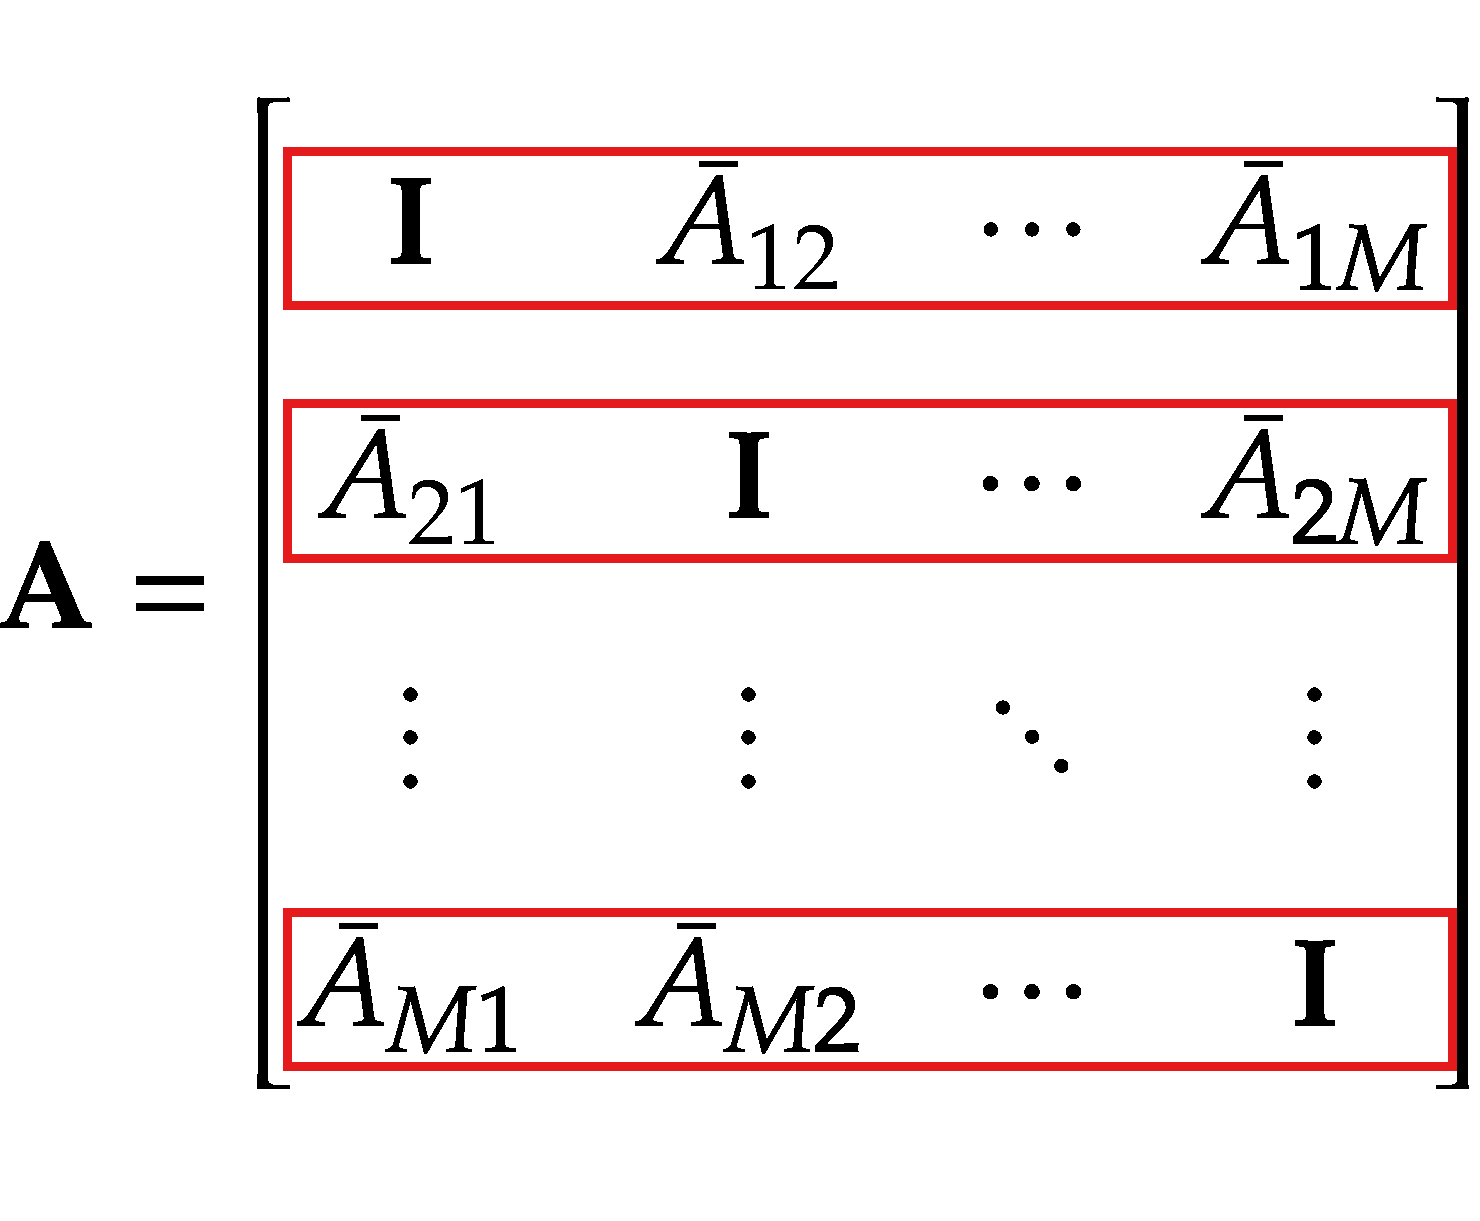
\includegraphics[width=\textwidth]{img/thread_block1D.pdf}
    \caption{1D}\label{fig:thread_block_1D}
  \end{subfigure}
  \begin{subfigure}[h]{0.33\textwidth}
    \centering
    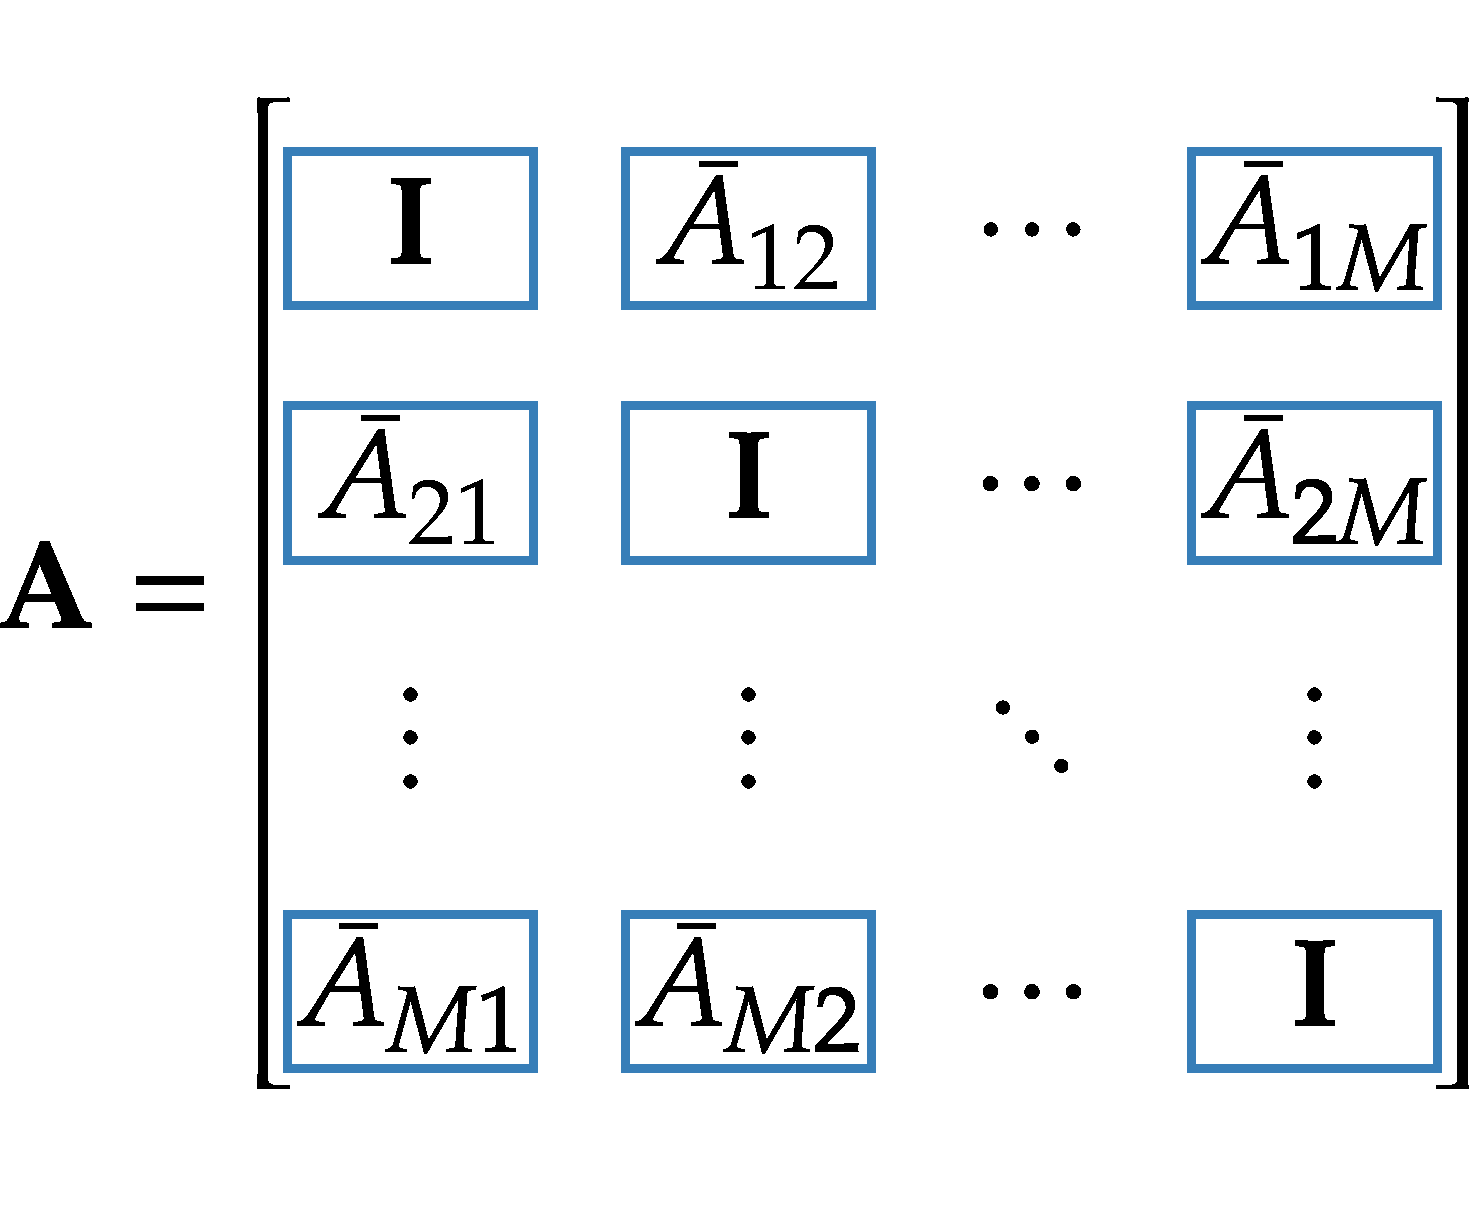
\includegraphics[width=\textwidth]{img/thread_block2D.pdf}
    \caption{2D}\label{fig:thread_block_2D}
  \end{subfigure}
  \caption[Illustration of 1D and 2D thread block dimensions for the system matrix.]{Illustration of 1D and 2D thread block dimensions for the system matrix. In the 1D case each thread is responsible for all interactions. For the 2D case each thread is only responsible for the interaction between a pair of fibers.}
  \label{fig:thread_block}
\end{figure}

The most straight forward approach is to use the one-dimensional thread block which means that the algorithm is parallelized with regard to a single fiber. In this case a single kernel invocation is responsible for multiple rows of the resulting linear system matrix, see Fig.~\ref{fig:thread_block_1D}. Additionally, this approach does not have any memory access conflict as each kernel only writes to the memory location belonging to its unique fiber. The potential disadvantage for a one-dimensional thread block, however, is that the resulting code can be more resource intensive for each single kernel and potentially hinder the performance on each multiprocessor.

For a two-dimensional thread block each kernel invocation is responsible for a pair of interacting fibers as shown in Fig.~\ref{fig:thread_block_2D}. While this decreases the necessary resources, it also requires atomic functions to handle the case when two threads try to update the right-hand side value for the same fiber. By using the so-called atomic functions CUDA streamlines and serializes the memory access. For example the \emph{atomicAdd} function in Listing~\ref{lst:pseudo_update_velocities} for the \emph{Update Velocities} step accumulates the contributions to a fiber from all the other fibers. This ensures that each update to the memory location is handled in a serial manner, guaranteeing the correct value in memory. Of course this implies a potential performance degradation, however, newer GPUs with new CUDA versions have been very well optimized to only have a minimal impact. Benchmarking for the rigid fibers simulation shows that using a two-dimensional thread block with the associated performance increases, outweigh the potential performance hit of using atomics.

Three-dimensional thread blocks are the maximum allowed dimensions for a CUDA thread block. They are a further extension of the two-dimensional thread block, as now each kernel invocation is not responsible for the complete interaction but only the interaction resulting from a specific point of the force expansion. This results in even more potential memory conflicts and also increases the total number of thread blocks which have to be distributed.

It is not clear, how exactly the performance is affected by each decision for the thread block dimension. Only trial-and-error benchmarking combined with metrics from CUDA can find the optimal setting for the specific algorithm. We will show in Sec.~\ref{subsec:bench_thread_block}, that for our GPU implementation the two-dimensional approach is the most efficient one.

\section{OpenMP}

The goal of this thesis is to implement a high performance rigid fiber simulation code on the GPU using CUDA. In order to better understand to what degree this goal is achieved, it is crucial to be able to do a fair comparison. The original serial implementation is not an ideal candidate as it does differ in a number of ways. First of all, it is purely serial and it does not take advantage of todays multicore CPUs. Furthermore, it is implemented in double precision, which is not suitable for the GPU used in this thesis. Finally, the primary focus of the original Fortran implementation was a correctly implemented algorithm and not performance.

For these reasons and in order to have a fairer comparison of the performance differences between the GPU and CPU implementation, a completely new parallel CPU code is also implemented. For the parallelization on the CPU the OpenMP library,~\cite{OpenMP}, was chosen.

After having implemented a parallel algorithm for the GPU, the conversion to the OpenMP-based CPU implementation was relatively straightforward. All optimizations done for the GPU implementation were also applied to the new CPU code when applicable. In order to parallelize the BLAS functions required for the linear solver the already included OpenBLAS library,~\cite{OpenBLAS}, was chosen. OpenBLAS is an open-source and highly optimized library and automatically parallelizes BLAS functions using pthreads across all available CPU cores. In contrast to the GPU implementation, the OpenMP version is only parallelized using a similar approach as the one-dimensional thread block on GPU as discussed in Sec.~\ref{subsec:parallel_thread_block}. This means that each core calculates the interactions for one fiber with all other fibers or put differently each core calculates the entire matrix row belonging to one fiber, as illustrated in Fig.~\ref{fig:thread_block_1D}. As the underlying number of independent threads is much lower on CPUs, different parallelization dimensions did not have an impact during testing.

The end results of the practical implementation for this thesis is a highly optimized CUDA implementation for NVIDIA GPUs and additionally a parallelized and optimized Fortran OpenMP implementation for CPUs. In the next chapter we will present a number of performance metrics and comparisons between the GPU and CPU implementations.


\chapter{Benchmarks}
\label{cha:benchmarks}

The previous chapter introduced the parallel implementation of the numerical algorithm using NVIDIA's CUDA framework. It presented a practical overview of the GPU implementation and discussed various strategies for optimizing the algorithm.

In this chapter we will present a number of benchmark tests. The main goal of the benchmarks is to measure the performance of the GPU implementation and compare it to the performance of the OpenMP-based CPU implementation. In addition to the comparison between the two different implementations, benchmark tests are also performed to investigate the different approaches for optimizing the code presented in the previous chapter.

\section{Methodology}

The methodology used for the benchmark suite is the same for all presented benchmarks. This ensures comparable results and the fairest comparison possible. A brief overview of the hardware and benchmark scheme used are described in the next sections.

\subsection{Hardware}

All benchmarks are run on the same workstation with specifications listed in Tab.~\ref{tab:workstation}. These hardware components can be considered a balanced system. This is done to come as close as possible to a fair comparison between the CPU and GPU, as comparing a high-end CPU against a low-end GPU would only be of limited value.

\begin{table}[htbp]
  \begin{center}
    \begin{tabulary}{0.7\textwidth}{LL}
      \toprule
      \multicolumn{2}{c}{Workstation} \\
      \midrule
      Processor & Intel Core i7 4770 \\
      Graphics & NVIDIA GTX 970 4GB \\
      RAM & 16GB DDR3 \\
      Operating System & Ubuntu Linux 12.04 LTS \\
      CUDA Driver & CUDA 6.5.16 \\
      \bottomrule
    \end{tabulary}
  \end{center}
  \caption{Benchmark hardware specification.}
  \label{tab:workstation}
\end{table}

The Intel Core i7 4770 processor is an 4-Core CPU based on Intel's Haswell Architecture. With its 8 parallel threads and $3.4$ GHz it was one of the top-of-line processor from 2013/14 and is currently still available for around $300\$$. The NVIDIA GTX 970 4GB is part of NVIDIA newest lineup of graphics cards based on the Maxwell Architecture. The main advantage of these new cards is the large memory of $4$ GB allowing for larger simulations. With a current price of slightly above $300\$$ it fills the middle price class for all Maxwell cards. Overall this can be considered to be a balanced system.

\subsection{Benchmark scheme}
\label{subsec:benchmark_scheme}

In order to generate statistically significant and reproducible execution times, all benchmarks tests for both the CPU and GPU implementation uses exactly the same run-scheme.

For each benchmark run we start with a configuration of M fibers randomly distributed in space. In order to exclude configurations where fibers overlap and/or intersect, the random process is modified such that there always is a fixed minimum distance between two fibers. Furthermore, in order to ensure a fair comparison between e.g. different linear solvers, the average distance between fibers are kept fixed for all runs independently of the number of fibers. As will be shown in Sec.~\ref{subsec:example_concentration_gmres}, the number of iterations of the iterative solvers depend on the average distance between the fibers. As the average distance become smaller, the condition number of the matrix increases and more iterations are needed for the iterative solver to converge. Thus by keeping the average distance between the fibers fixed, we minimize the influence of the number of iterations in the iterative solver on the execution time.

Using the semi-random fiber configuration, the simulation is run for 10 time steps. To avoid remaining outliers in the configuration potentially causing variations in the timings the first time step is excluded. The first time step is thus used as a simple warmup step for the simulation. So, the final average time for each run is measured using the final $9$ time steps.

To measure how the execution time depends on the number of fibers in the simulation, all tests are run with varying number of fibers starting from $100$ fibers up to $2000$ fibers using an increment of $100$.

\begin{listing}[htbp]
  \centering
  \inputminted[mathescape,
    linenos,
    numbersep=5pt,
    fontsize=\footnotesize,
    frame=lines,
    framesep=2mm]{c}{lst/benchmark_scheme.lst}
  \caption{Pseudocode for benchmark scheme.}
  \label{lst:pseudo_benchmark}
\end{listing}

In addition, every run is repeated a number of times where each run uses a new random fiber configuration. The final execution time is computed as the average time over the total number of runs. The execution time is measured using the built-in CUDA timing events for the GPU implementation and the Fortran \emph{SYSTEM\_CLOCK} function for the CPU implementation.

To further improve the statistical significance of the result the benchmark scheme dynamically adjusts the number of runs performed for each test. If the relative standard error (RSE) of the measured timings collected is too high after a minimum number of runs, more runs are scheduled. This repeats until the relative standard error falls below $20\%$ and reliable timings have been obtained.  The algorithm for producing the benchmark results is illustrated using pseudocode in Listing~\ref{lst:pseudo_benchmark}. 

\section{Optimizations}
\label{sec:bench_optimization}

We now look at the performance results for the different optimizations strategies previously outlined in Sec.~\ref{sec:parallel_optimizations}. Where applicable, the results will be compared between the OpenMP and the CUDA version of the algorithm.

\subsection{Numeric vs. Analytic Integration}
\label{subsec:bench_numeric_vs_analytic}

The first benchmark tests the performance of the two different approaches to compute the inner integral in Eqn.~\eqref{eq:inner_integral}. It can be solved either numerically or analytically. Fig.~\ref{fig:openmp_num_vs_anal} illustrates the performance timings for the \emph{Assemble System} step of the parallel OpenMP version. Inline with the observations made by the authors of the original serial implementation,~\cite{Tornberg2006}, analytical integration is always faster to use than numerical integration.
\begin{figure}[htbp]
  \centering
  \begin{tikzpicture}
    \begin{axis}[
	width=0.77\textwidth,
      xlabel={Number of fibers},
      ylabel={Execution time (sec)},
      enlarge y limits=true,
      enlarge x limits=true,
      unbounded coords=discard,
      xmode=log,
      ymode=log,
      grid=major,
      ]
      \addplot[color=set11,mark=*,mark options={fill=white}, very thick] table[x=X,y=ASSEMBLE_SYSTEM] {benchmarks/openmp_direct_numerical.csv};
      \addplot[color=set12,mark=square*,mark options={fill=white}, very thick] table[x=X,y=ASSEMBLE_SYSTEM] {benchmarks/openmp_direct_analytical.csv};

      \legend{Numerical, Analytical}
    \end{axis}
  \end{tikzpicture}
  \caption[Benchmark computing inner integral on CPU.]{Benchmark comparing numerical and analytical integration of the inner integral in Eqn.~\eqref{eq:inner_integral} using OpenMP.}
  \label{fig:openmp_num_vs_anal}

  \begin{tikzpicture}
    \begin{axis}[
	width=0.77\textwidth,
      xlabel={Number of fibers},
      ylabel={Execution time (sec)},
      enlarge y limits=true,
      enlarge x limits=true,
      unbounded coords=discard,
      xmode=log,
      ymode=log,
      grid=major,
      ]
      \addplot[color=set11,mark=*,mark options={fill=white}, very thick] table[x=X,y=assemble_system] {benchmarks/cuda_bicgstab_numerical_2D.csv};
      \addplot[color=set12,mark=square*,mark options={fill=white}, very thick] table[x=X,y=assemble_system] {benchmarks/cuda_bicgstab_analytical_2D.csv};

      \legend{Numerical, Analytical}
    \end{axis}
  \end{tikzpicture}
  \caption[Benchmark computing inner integral on GPU.]{Benchmark comparing numerical and analytical integration of the inner integral in Eqn.~\eqref{eq:inner_integral} using CUDA.}
  \label{fig:cuda_num_vs_anal}

\end{figure}

In contrast to the expected and obtained results using the OpenMP implementation, the CUDA implementation shows a different picture. When we look at the corresponding graph for the CUDA implementation in Fig.~\ref{fig:cuda_num_vs_anal}, we observe that the results are reversed. Numerical integration outperforms the analytical integration by a large margin that even increases with the number of fibers.

The reason for this result lies in the scheduling and execution of work on the GPU. All code inside a thread block (more precisely a warp) is always executed in lockstep. This means that each line of code is executed for each thread in parallel. However, if the code encounters a branch in the execution path, like a simple \emph{if} statement, the threads diverge. First, all threads for which the condition is true are executed while the other threads have to wait. Then all threads for which the condition is false are executed while the others are not used. Finally, after all divergent code paths have been executed the code continues in lockstep. This issue is referred to as branch divergence and should be avoided as much as possible when writing parallel GPU Code,~\cite{CudaBestPracticeGuide}.

To confirm that branch divergence is the reason for the slowdown of the analytic integration version of the GPU implementation we look at the metrics of the CUDA profiler \emph{nvprof}. The metric \emph{Warp Execution Efficency} shows the ratio of the average active threads per warp to the maximum number of threads per warp. The metrics for both the numerical and analytical integration can be seen in Tab.~\ref{tab:branch_divergence}.

\begin{table}[htbp]
  \begin{center}
    \begin{tabulary}{0.7\textwidth}{LR}
      \toprule
      Algorithm & warp\_execution\_efficiency \\
      \midrule
      Numerical & $99.01\%$ \\
      Analytical & $53.79\%$ \\
      \bottomrule
    \end{tabulary}
  \end{center}
  \caption[Warp Execution Efficiency of Numerical vs. Analytical Integration.]{CUDA performance metric \emph{Warp Exection Efficiency} comparison for the numerical and analytical integration of the inner integral in Eqn.~\eqref{eq:inner_integral}.}
  \label{tab:branch_divergence}
\end{table}

On the one hand the numerical integration is almost $100\%$ efficient, which means that all warps execute in complete lockstep. The analytical integration on the other hand is only $50\%$ efficient, meaning that most of the time only half of the threads actually perform work while the other half is just waiting. This results in the observed performance difference. As already discussed in Sec.~\ref{subsec:numeric_analytic} the analytical evaluation of the inner integral potentially suffers from numerical instabilities. Closer inspection of the source code reveals that the steps taken to minimize these instabilities are responsible for the branch divergence and explains the decrease in performance on the GPU. The steps involve a simple \emph{if} statement, that switches between two code path depending on how far apart two fibers are. Unfortunately, this workaround is unavoidable to ensure numeric stability.

\subsection{Shared memory}
\label{subsec:bench_shared_memory}

Since the data transfer between the compute units and the global memory is slow, the second optimization strategy is to try to use shared memory to reduce the amount of data that has to be transferred. For this each Streaming Multiprocessor (SM) has a small amount of locally shared memory. This memory can be accessed from all threads on the SM. If data can be shared, it only has to be transferred from global to shared memory once. Afterwards, in can be accessed from the faster local memory.

During testing and benchmarking the shared memory implementation of the \emph{Assemble System} step described in Sec.~\ref{subsec:shared_memory}, showed no effect on the performance. Even though data can theoretically be shared among different threads it does not result in shorter execution times.

The reason for this is that the \emph{Assemble System} step is compute bound and not memory bound. This means that the time it takes to execute the computations, e.g. evaluating the integrals, takes substantially longer than reading and writing to global memory. This can be explained by looking at the two-dimensional thread block version, where each kernel is responsible for a pair of fibers. Each kernel only needs to read $4$ vectors from global memory, the position and orientation of both fibers. Assuming single precision this is a total of just $4 * 3 * 4~\text{bytes} = 48~\text{bytes}$ per kernel invocation.

While waiting for this data from global memory, CUDA is able to quickly switch between different sets of threads and continue the computation there. Thus the only waiting time occurs when the very first set of data has to be loaded. Once the first amount of data has arrived, computations can be performed using it. While the long running computations are executed, other threads can start issuing data loading requests. When the first computation is done and the next set of threads is executed, the data has already been read from memory. As there was no advantage in using shared memory in the compute bound \emph{Assemble System} step, we opted for the simpler implementation without it in all subsequent simulations.

\subsection{Thread block dimension}
\label{subsec:bench_thread_block}

The final optimization strategy studied is the Thread Block Dimension on the GPU. Choosing the best option is a trade-off between the resources used and the overhead caused by an increased amount of memory writes to the same location. Writing to the same memory location from different threads would result in undefined behavior and avoiding this requires the usage of potentially slow atomic functions.

The results in Fig.~\ref{fig:bench_cuda_thread_blocks} indicate that the best option for this particular GPU is a two-dimensional thread block. The three-dimensional thread block is always slower and the performance gap grows with the number of fibers. The reason for this performance gap is the increased usage of atomics in the three-dimensional case. The overall usage of atomic functions can be inspected with the NVIDIA profiler \emph{nvprof} and the profiling metric \emph{Atomic Transactions}. This metric simply counts the total number of atomic transactions performed when atomic functions are used. Tab.~\ref{tab:atomic_transactions} lists the \emph{Atomic Transactions} counts for both the two-dimensional and three-dimensional thread block implementation running an example with $2000$ fibers. The required \emph{Atomic Transactions} in the three-dimensional case are almost two times larger than for the two-dimensional case. These additional transactions incur a performance penalty, because they serialize the access to memory and threads have to wait while other threads finish writing to memory.

\begin{figure}[htbp]
  \centering
  \begin{tikzpicture}
    \begin{axis}[
      xlabel={Number of fibers},
      ylabel={Execution time (sec)},
      enlarge y limits=true,
      enlarge x limits=true,
      unbounded coords=discard,
      xmode=log,
      ymode=log,
      grid=major,
      ]
      \addplot[color=set11,mark=*,mark options={fill=white}, very thick] table[x=X,y=assemble_system] {benchmarks/cuda_magma_numerical_1D.csv};
      \addplot[color=set12,mark=square*,mark options={fill=white}, very thick] table[x=X,y=assemble_system] {benchmarks/cuda_magma_numerical_2D.csv};
      \addplot[color=set13,mark=triangle*,mark options={fill=white}, very thick] table[x=X,y=assemble_system] {benchmarks/cuda_magma_numerical_3D.csv};

      \legend{1D, 2D, 3D}
    \end{axis}
  \end{tikzpicture}
  \caption[Benchmarking thread block dimensions.]{Benchmark comparing different parallelization options of the \emph{Assemble System} step using thread block dimensions as described in Sec.~\ref{subsec:parallel_thread_block}. }
  \label{fig:bench_cuda_thread_blocks}
\end{figure}

\begin{table}[htbp]
  \begin{center}
    \begin{tabulary}{0.7\textwidth}{LR}
      \toprule
      Algorithm & atomic\_transactions \\
      \midrule
      2D & $1,269,325$ \\
      3D & $2,350,670$ \\
      \bottomrule
    \end{tabulary}
  \end{center}
  \caption[Atomic transactions of 2D vs. 3D thread block dimensions.]{CUDA performance metric \emph{Atomic transactions} comparison for the 2D and 3D thread block dimensions parallelization of the \emph{Assemble System} step.}
  \label{tab:atomic_transactions}
\end{table}

Fig.~\ref{fig:bench_cuda_thread_blocks} also shows that the one-dimensional approach is slower than both the two-dimensional and three-dimensional approach. However, it appears to scale linearly whereas the other two scale quadratically with the number of fibers. It can already be observed that the performance of the one-dimensional thread block becomes faster than the three-dimensional thread block for close to $2000$ fibers. Unfortunately, the hardware of the workstation does not have enough memory to simulate more fibers, allowing the one-dimensional approach to overtake the two-dimensional approach. Thus at least for our simulation we always use the two-dimensional approach.

\section{Linear solvers}
\label{sec:bench_linear_solvers}

Next we compare the performance for different linear solvers. The time required for solving the linear system can be a very large part of the overall runtime, depending choice of solver and the fiber configuration as discussed in Sec.~\ref{sec:algorithm_summary}. It is therefore very important to find the optimal solver in order to arrive at the best performing algorithm overall. We explore both direct and iterative solvers.

\subsection{Direct solver vs iterative solver on CPU}
On the CPU side we use the direct solver provided by the fully parallelized OpenBLAS library. For GMRES we use the single precision Fortran implementation from Frayssé et al.,~\cite{Fraysse2003}, which takes extensive advantage of the underlying BLAS functions parallelized by OpenBLAS. 

If we compare the execution time when using GMRES to using a direct solver, we observe that GMRES is faster by a wide margin, see Fig.~\ref{fig:bench_openmp_solvers}. This was also observed in the original serial version of the code,~\cite{Tornberg2006}.

\begin{figure}[htbp]
  \centering
  \begin{tikzpicture}
    \begin{axis}[
      xlabel={Number of fibers},
      ylabel={Execution time (sec)},
      enlarge y limits=true,
      enlarge x limits=true,
      unbounded coords=discard,
      xmode=log,
      ymode=log,
      grid=major,
      ]
      \addplot[color=set11,mark=*,mark options={fill=white}, very thick] table[x=X,y=SOLVE_SYSTEM] {benchmarks/openmp_direct_numerical.csv};
      \addplot[color=set12,mark=square*,mark options={fill=white}, very thick] table[x=X,y=SOLVE_SYSTEM] {benchmarks/openmp_gmres_numerical.csv};

      \legend{Direct Solver, GMRES}
    \end{axis}
  \end{tikzpicture}
  \caption[Benchmark linear solvers on CPU.]{Benchmarking comparing linear solvers on the CPU. The direct solver is provided by OpenBLAS,~\cite{OpenBLAS}, and iterative GMRES solver by Frayssé et al.,~\cite{Fraysse2003}.}
  \label{fig:bench_openmp_solvers}
\end{figure}

From an advantage of just ${\sim}40×$ for $1000$ fibers this increases to ${\sim}300×$ for the maximum number of $2000$ fibers. As expected we can also see in Fig~\ref{fig:bench_openmp_solvers} that GMRES clearly scales better with the number of fibers than the direct solver.

\subsection{Fiber concentration effect on GMRES iterations}
\label{subsec:example_concentration_gmres}

During the initial benchmark tests we observed large differences in the execution time for different fiber configurations when using GMRES. The reason for this was that for some runs, especially for a high concentration of fibers, GMRES required a large number of iterations to converge.

When the fiber concentration increases, the average distance between the fibers decreases. To investigate how the number of GMRES iterations depend on the concentration of fibers, we perform a number of runs where the average pair-wise distance between the fibers varies from $0.01$ to $40$.

\begin{figure}[htbp]
  \centering
  \begin{tikzpicture}
    \begin{axis}[
      xlabel={Concentration},
      ylabel={GMRES iterations},
      width={0.8\textwidth},
      unbounded coords=discard,
      xmode=log,
      ymode=log,
      grid=major,
      enlarge y limits=true,
      enlarge x limits=true,
      ]

      \addplot[color=set11, mark=*,mark options={fill=white}, very thick] table[x=Concentration,y=Average,col sep=comma] {charts/concentration_gmres.csv};

    \end{axis}
  \end{tikzpicture}
  \caption[Effect of fiber concentration on GMRES iterations.]{Effect of fiber concentration on GMRES iterations. The number of GMRES iterations increases dramatically when the distance between the fibers is small.}
  \label{fig:concentration_gmres}
\end{figure}

In Fig.~\ref{fig:concentration_gmres} the result is presented. We see that for a decrease in the pair-wise distance, the number of iterations increases quite rapidly. To find the reason for this we have to look at Eqn.~\eqref{eq:inner_integral} which forms the basis for the entries in the matrix. When evaluating the integral the Greens function $\mathbf{G}(\mathbf{R})$ defined in Eqn.~\eqref{eq:green_function} has to be computed. Since $\mathbf{G}(\mathbf{R}) \sim 1/\mathbf{R}$ where $\mathbf{R}$ is given by the distance between fibers, some of the entries in the matrix become very large when the distance is small. The consequence is a growth in the condition number of the matrix and thus an increase in the number of GMRES iterations is required for convergence. This is the reason why we keep the concentration of fibers fixed for all benchmark runs, as described in Sec.~\ref{subsec:benchmark_scheme}.

The result presented above is also important to keep in mind when performing long running fiber simulations. Here, the probability that any two fibers get close to each other is very high. If this is the case, solving the system by GMRES will take longer than expected. In practice it might be more beneficial to switch to the direct solver as it has a predictable runtime. This is especially true using the GPU implementation as the difference in execution time between direct and iterative solver is relatively small. This will be discussed further in the next section.

\subsection{Direct solver vs. iterative solver on GPU}

We will now look at the performance of the direct solver compared to the iterative solvers on the GPU. We use a direct solver provided by the MAGMA library and the iterative solvers, BiCGStab and GMRES, from the ViennaCL library. The benchmark results are illustrated in Fig.~\ref{fig:bench_cuda_solvers}.

\begin{figure}[htbp]
  \centering
  \begin{tikzpicture}
    \begin{axis}[
      xlabel={Number of fibers},
      ylabel={Execution time (sec)},
      enlarge y limits=true,
      enlarge x limits=true,
      unbounded coords=discard,
      xmode=log,
      ymode=log,
      grid=major,
      ]
      \addplot[color=set11,mark=*,mark options={fill=white}, very thick] table[x=X,y=solve_system] {benchmarks/cuda_magma_numerical_2D.csv};
      \addplot[color=set12,mark=square*,mark options={fill=white}, very thick] table[x=X,y=solve_system] {benchmarks/cuda_bicgstab_numerical_2D.csv};
      \addplot[color=set13,mark=triangle*,mark options={fill=white}, very thick] table[x=X,y=solve_system] {benchmarks/cuda_gmres_numerical_2D.csv};

      \legend{Direct Solver, BiCGStab, GMRES}
    \end{axis}
  \end{tikzpicture}
  \caption[Benchmark linear solvers on GPU.]{Benchmarking comparing linear solvers on the GPU. The direct solver is provided by MAGMA,~\cite{MagmaDocumentation}, and iterative solvers, BiCGStab and GMRES, by ViennaCL,~\cite{ViennaCLRupp2010}.}
  \label{fig:bench_cuda_solvers}
\end{figure}

The fact that iterative solvers are faster than a direct solver holds true also for the GPU. However, compared to the results on the CPU the difference between the performance of the direct solver and the iterative solvers is not as large. At close to $2000$ fibers the iterative solvers are only about $25×$ faster than the direct solver as compared to the result on the CPU where GMRES was $300×$ faster than the direct solver. Looking at the difference between the two iterative solvers, BiCGStab and GMRES they perform almost exactly the same. Any small differences can be attributed to small measuring uncertainties. 

Regardless of these clear results, it is always important to keep in mind, that this particular performance ratio only holds true for the specific fiber concentration which was benchmarked. For other concentrations the iterative solvers might need more iterations to find the solution and might even perform worse than the linear solver.

\section{Individual steps of the algorithm}

The next benchmark explores the relative time taken by each step of the algorithm described in Sec.~\ref{sec:algorithm_summary}~and Sec.~\ref{sec:kernels}. This yields valuable insight into the time allocation of the overall execution time, thereby helping to figure out which steps are the best ones to optimize. The results for the OpenMP implementation can be seen in Fig.~\ref{fig:bench_openmp_steps} and for the CUDA implementation in Fig.~\ref{fig:bench_cuda_steps}. On the CPU the \emph{Assemble System} and \emph{Update Velocities} steps solve the inner integral in Eqn.~\eqref{eq:inner_integral} analytically. On the GPU we use a purely numerical approach. The reason for choosing different approaches for evaluating the inner integral is to use the fastest version of the algorithm on both the CPU and GPU, see Sec.~\ref{subsec:bench_numeric_vs_analytic}.

\begin{figure}[htbp]
  \centering
  \begin{tikzpicture}
    \begin{axis}[
	width=0.77\textwidth,
      xlabel={Number of fibers},
      ylabel={Execution time (sec)},
      stack plots=y,
      ymin=0,ymax=50,
      xmin=0,xmax=2000,
      ]
      \addplot[color=set19,mark=*,mark options={fill=white}, very thick, stack plots=false] table[x=X,y=TOTAL] {benchmarks/openmp_gmres_analytical.csv};
      \addplot[color=set11,fill=set11_light,ultra thin,area style] table[x=X,y=ASSEMBLE_SYSTEM] {benchmarks/openmp_gmres_analytical.csv} \closedcycle;
      \addplot[color=set12,fill=set12_light,ultra thin,area style] table[x=X,y=SOLVE_SYSTEM]{benchmarks/openmp_gmres_analytical.csv} \closedcycle;
      \addplot[color=set13,fill=set13_light,ultra thin,area style] table[x=X,y=UPDATE_VELOCITIES] {benchmarks/openmp_gmres_analytical.csv} \closedcycle;
      \addplot[color=set14,fill=set14_light,ultra thin,area style] table[x=X,y=UPDATE_FIBERS] {benchmarks/openmp_gmres_analytical.csv} \closedcycle;

      \legend{Total, Assemble System, Solve System, Update Velocities, Update Fibers}
    \end{axis}
  \end{tikzpicture}
  \caption[Benchmark individual steps on CPU.]{Benchmark comparing the execution for each individual step of the algorithm using the OpenMP-based CPU implementation.}
  \label{fig:bench_openmp_steps}

  \begin{tikzpicture}
    \begin{axis}[
	width=0.77\textwidth,
      xlabel={Number of fibers},
      ylabel={Simulation time (sec)},
      stack plots=y,
      ymin=0,ymax=1.4,
      xmin=0,xmax=2000,
      ]
      \addplot[color=set19,mark=*,mark options={fill=white}, very thick, stack plots=false] table[x=X,y=total] {benchmarks/cuda_gmres_numerical_2D.csv};
      \addplot[color=set11,fill=set11_light,ultra thin,area style] table[x=X,y=assemble_system] {benchmarks/cuda_gmres_numerical_2D.csv} \closedcycle;
      \addplot[color=set12,fill=set12_light,ultra thin,area style] table[x=X,y=solve_system]{benchmarks/cuda_gmres_numerical_2D.csv} \closedcycle;
      \addplot[color=set13,fill=set13_light,ultra thin,area style] table[x=X,y=update_velocities] {benchmarks/cuda_gmres_numerical_2D.csv} \closedcycle;
      \addplot[color=set14,fill=set14_light,ultra thin,area style] table[x=X,y=update_fibers] {benchmarks/cuda_gmres_numerical_2D.csv} \closedcycle;

      \legend{Total, Assemble System, Solve System, Update Velocities, Update Fibers}
    \end{axis}
  \end{tikzpicture}
  \caption[Benchmark individual steps on GPU.]{Benchmark comparing the execution for each individual step of the algorithm using the CUDA-based GPU implementation.}
  \label{fig:bench_cuda_steps}
\end{figure}

The results for the OpenMP implementation, Fig.~\ref{fig:bench_openmp_steps}, show that for $2000$ fibers the \emph{Assemble System} step is responsible for $78\%$ and the \emph{Update Velocities} step for $21\%$ of the overall time. The two other steps \emph{Solve System} and \emph{Update Fibers} barely register with just $1\%$. However, as discussed in the previous Sec.~\ref{sec:bench_linear_solvers} this only holds true for sufficiently low concentrations of fibers.

\begin{figure}[htbp]
  \centering

\end{figure}

For the CUDA implementation, Fig.~\ref{fig:bench_cuda_steps} shows that the \emph{Assemble System} step remains the largest block with $72\%$ of the time. However, now the \emph{Solve System} step takes $20\%$ of the time and \emph{Update Velocites} drops to just $7\%$. The \emph{Update Fibers} step is also negligible here with below $1\%$.

This difference between the CPU and GPU implementation in the relative time between the steps can be attributed to the comparatively slow GMRES implementation on the GPU. In absolute terms for $2000$ fibers both the CPU and GPU take ${\sim}0.25$ seconds for solving the system. But, when transferring the same relative distribution from the CPU to GPU this makes the GPU GMRES implementation $40×$ too slow. The other steps all perform relatively better.

The reason for this most likely lies in the non-optimized code for the GMRES solver in ViennaCL. The authors openly state that the major goal for their library is easy of use and not pure performance,~\cite{ViennaCLRupp2010}. The parallel BLAS functions from OpenBLAS on the other hand have been highly optimized and tested for a long time.

This point is reinforced if we look at the same timings for the linear solvers. Here the absolute time for \emph{Solve System} step on the GPU is just ${\sim}7$ seconds compared to the ${\sim}76$ seconds on the CPU. Again transferring the relative distribution from the CPU to the GPU yields just a small factor of ${\sim}1.4×$. This illustrates that the highly optimized code of the MAGMA library performs roughly on the same level as the optimized code from OpenBLAS.

\section{GPU vs. CPU}

The final benchmark compares the CPU and GPU performance. How to make a fair comparison of the simulation performance between the CPU and GPU is a hotly debated topic in the research literature,~\cite{Gregg2011}\cite{Lee2010}. The underlying architectures of the two approaches are completely different and thus hard to compare. There are approaches where the relative performance is extrapolated from the underlying FLOPs by taking processor count, frequency and memory bandwidth into account,~\cite{Lee2010}. However, due to intricate hardware details this approach is not applicable to all scenarios. Thus in the super computing community metrics like performance-per-dollar or even performance-per-watt have become the main focus,~\cite{Kamil2008}.

Exploring this question in more detail is out of the scope of this thesis. Nevertheless we try to make a best effort to do fair comparison between the CPU and the GPU performance. In order to come as close as possible given these complexities and constraints, we use a modern CPU and GPU which can be considered a balanced system at the time of writing. Additionally, we implemented a parallel OpenMP version. It is directly based on the parallel CUDA version with the sole purpose to have as few difference between the two implementations as possible. Furthermore, the final benchmark uses the fastest possible version of the algorithms as determined by the performed benchmarks.

\begin{figure}[htbp]
  \centering
  \begin{tikzpicture}
    \begin{axis}[
      xlabel={Number of fibers},
      ylabel={Execution time (sec)},
      enlarge y limits=true,
      enlarge x limits=true,
      unbounded coords=discard,
      xmode=log,
      ymode=log,
      grid=major,
      ]

      \addplot[color=set11,mark=*,mark options={fill=white}, very thick] table[x=X,y=total] {benchmarks/cuda_gmres_numerical_2D.csv};
      \addplot[color=set11_light,mark=square*,mark options={fill=white}, very thick] table[x=X,y=total] {benchmarks/cuda_magma_numerical_2D.csv};
      \addplot[color=set12,mark=triangle*,mark options={fill=white}, very thick] table[x=X,y=TOTAL] {benchmarks/openmp_gmres_analytical.csv};
      \addplot[color=set12_light,mark=diamond*,mark options={fill=white}, very thick] table[x=X,y=TOTAL] {benchmarks/openmp_direct_analytical.csv};

      \legend{CUDA GMRES, CUDA Direct, OpenMP GMRES, OpenMP Direct}
    \end{axis}
  \end{tikzpicture}
  \caption[Benchmark overall execution time.]{Benchmark comparing overall execution time for OpenMP and CUDA. Both the CPU and GPU implementation are run using the fastest algorithm as determined in Sec~\ref{sec:bench_optimization} and each implementation is tested with a direct and iterative solver. The CUDA-based GPU implementation outperforms the OpenMP-based CPU implementation by ${\sim}40×$.\looseness=-1}
  \label{fig:overall}
\end{figure}

The results for the average time required to take a single time step is illustrated in Fig.~\ref{fig:overall}. For OpenMP the algorithm uses the analytical integration of the inner integral. For CUDA, we used the numerical integration and the thread block dimension was chosen to be two-dimensional.

The required simulation time on the GPU outperforms the CPU by a wide margin. The GPU version is faster for any number of fibers that we are able to test. The speedup factors for the tested versions are listed in Tab~\ref{tab:overall_speedup}. CUDA maintains a relative performance of ${\sim}40×$. The only advantage the CPU version has is the potentially larger memory as 4GB on the GPU limits the number of fibers to roughly $2000$. So for more fibers than $2000$, OpenMP is currently the only option.

\begin{table}[htbp]
  \begin{center}
    \begin{tabulary}{\textwidth}{lRRRR}
      \toprule
      M = 2000 & OpenMP Direct & OpenMP GMRES & CUDA Direct & CUDA GMRES \\
      \midrule
      OpenMP Direct & $1×$  & $—$   & $—$ & $—$ \\
      OpenMP GMRES  & $3×$  & $1×$  & $—$ & $—$ \\
      CUDA Direct   & $16×$ & $6×$  & $1×$ & $—$ \\
      CUDA GMRES    & $99×$ & $39×$ & $6×$ & $1×$ \\
      \bottomrule
    \end{tabulary}
  \end{center}
  \caption[Speedup factors for overall execution time.]{The speedup factors for the overall execution time of a simulation with $2000$ fibers for the CPU and GPU implementation. In case of a direct solver the GPU implementation shows a speedup of $16×$ compared to the CPU implementation. Comparing the two GMRES versions, the CUDA-based GPU implementation outperforms the OpenMP-based CPU implementation by $39×$.}
  \label{tab:overall_speedup}
\end{table}

We acknowledge that these numbers and performance increases are not necessarily fair. A different CPU and GPU combination from the one used in this thesis might perform differently. However, the relative performance should stay roughly the same. In the end, the only thing that really matters for the researcher working with rigid fibers is the time it takes to simulate large systems on the available workstation. There is no need to wait for computing time at a large computing cluster. Instead simulation can be run simply on a desktop computer allowing to rapidly iterate on the tests. The observed performance increase of $40×$ is comparable to a difference between a whole day of waiting for the simulation results and a quick $30$ minutes result. The saved time also translates directly into the ability to simulate many more fibers than before. Using the original serial implementation the largest simulation possible in a reasonable time frame where around $500$ to $800$ fibers. Now one single time step with $2000$ fibers takes at most $8$ seconds on the GPU. Therefore the implementation on the GPU and the optimizations of the simulation code is of great value to the research of rigid fiber simulations.


\chapter{Numerical experiments}
\label{cha:experiments}

The previous chapter showed how much faster the GPU implementation is compared to the same algorithm implemented on the CPU. This significant increase in performance allows for new numerical experiments.

In this chapter we will present results from a number of experiments performed to explore the numerical precision of the implementation and to validate the results against prior research. 

We begin by looking at tumbling orbits, a very delicate experiment requiring good numerical precision. Next we reproduce a very interesting physical phenomenon of letting a spherical cloud of fibers sediment and validate our results against similar experiment by others. Furthermore, we will have a brief exploration of the effects of the number of fibers and the concentration of fibers on the spherical cloud simulation. All experiments are run with the new GPU algorithm  implemented in the thesis. The linear system is solved using the direct solver from MAGMA in order to avoid variations in the run time.

\section{Tumbling orbits}
\label{sec:example_ring}

To verify that the single precision GPU implementation is able to replicate the result using the original double precision code, we perform a very simple experiment where a small number of fibers are set up with perfectly symmetrical positions and orientations. Initially, all fibers are evenly distributed on a circle and aligned vertically with gravity. During the simulation, while sedimenting, the fibers begin to rotate from their vertical orientation towards a horizontal position. Afterwards, they continue rotating back into the vertical position. This motion is referred to as a tumbling motion and as long as there are no disturbances or numerical precision issues it repeats forever.

This simple but very interesting problem has also been simulated by Gustavsson and Tornberg~\cite{Gustavsson2009}. Additionally an even more simplified version with only two fibers was studied both numerically and experimentally by Jung et al.~\cite{Jung2006}. This example is thus ideally suited to test and verify the numerical precision of the GPU implementation. A visualization of the result using the GPU code for $16$ fibers evenly distributed around a circle with a radius of $0.55$, is shown in Fig.~\ref{fig:ring_simulation}.

\begin{figure}[!htbp]
  \centering
  \begin{subfigure}[h]{0.45\textwidth}
    \centering
    \includegraphics[width=\textwidth]{img/ring_00000.pdf}
    \caption{$t=0$}\label{fig:ring_simulation_1a}
  \end{subfigure}
  \begin{subfigure}[h]{0.45\textwidth}
    \centering
    \includegraphics[width=\textwidth]{img/ring_00015.pdf}
    \caption{$t=15$}\label{fig:ring_simulation_1b}
  \end{subfigure}
  \begin{subfigure}[h]{0.45\textwidth}
    \centering
    \includegraphics[width=\textwidth]{img/ring_00030.pdf}
    \caption{$t=30$}\label{fig:ring_simulation_1c}
  \end{subfigure}
  \begin{subfigure}[h]{0.45\textwidth}
    \centering
    \includegraphics[width=\textwidth]{img/ring_00045.pdf}
    \caption{$t=45$}\label{fig:ring_simulation_1d}
  \end{subfigure}
  \caption[Visualization of tumbling orbits.]{Visualization of tumbling orbits. Small number of perfectly symmetrically distributed fibers around a circle are allowed to sediment due to gravity. The fibers perform a periodical motion alternating between a vertical and horizontal orientation in the direction to gravity.}
  \label{fig:ring_simulation}
\end{figure}

Initially, the fibers are aligned vertically and are sedimenting with the maximum velocity. As they rotate into the horizontal orientation the velocity decreases and reaches its minimum once the fibers are perpendicular to the direction of gravity. Afterwards on their way back to vertical orientation the velocity increases again.

Fig.~\ref{fig:ring_sedimentation_velocity} shows a graph of the sedimentation velocity of a single fiber over time for both the single precision GPU code and the original double precision Fortran code. As the same force acts on all fibers and they perform the same motion they all have the same sedimentation velocity. For this particular setup the maximum velocity is $~3.8$ and the minimum velocity is $~2.2$. The graphs clearly shows the periodical rotation the fiber perform. This result perfectly captures the expected result obtained from prior simulation and experiments. The difference in velocity between the two implementations is of the order $10^{-4}$. Hence, even for this delicate experiment, where a small disturbance will cause a deviation from the periodic orbit, the single precision accuracy is sufficient.

\begin{figure}[!htbp]
  \centering
  \begin{tikzpicture}
    \begin{axis}[
      xlabel={Timestep},
      ylabel={Velocity},
      height={207pt},
      unbounded coords=discard,
      xmin=0,xmax=200,
      ymin=-4,ymax=-2,
      ]

      \addplot[color=set12, very thick] table[x=Timestep,y=Single] {charts/ring_sedimentation.csv};
      \addplot[color=set11, loosely dashed, ultra thick] table[x=Timestep,y=Double] {charts/ring_sedimentation.csv};
    \end{axis}
  \end{tikzpicture}
  \caption[Comparison of sedimentation velocity for single- and double-precision simulation.]{Comparison of sedimentation velocity for single precision (solid line) and double precision (dahsed line) simulation.}
  \label{fig:ring_sedimentation_velocity}
\end{figure}

\section{Sedimenting of a spherical cloud}
\label{sec:example_sphere}

The next example is a more chaotic system with a large number of interacting fibers. In the numerical experiment $2000$ fibers are initially distributed in the form of a spherical cloud. Both their positions and orientations are random inside the cloud. Due to gravity the cloud will sediment. This experiment has been studied in several papers, e.g.~\cite{Bulow2015}\cite{Metzger2007}\cite{Park2010}. It is especially interesting because the observed results only occur if enough fibers are simulated. Our GPU simulation is able to efficiently handle up to $2000$ fibers and is thus ideally suited for studying this example.

\begin{figure}[!htbp]
  \centering
  \begin{subfigure}[h]{0.4\textwidth}
    \centering
    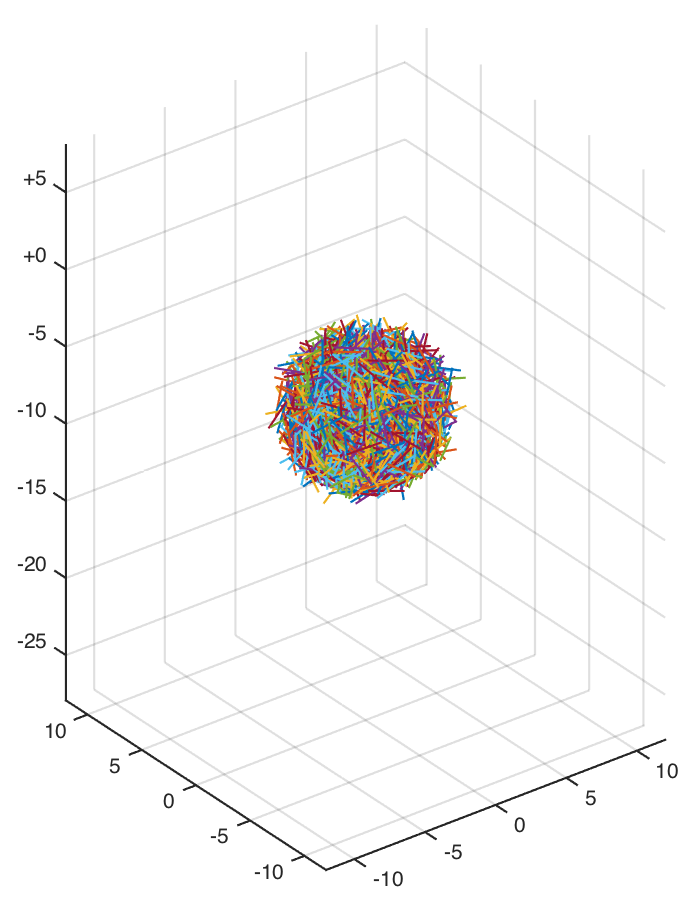
\includegraphics[width=\textwidth]{img/state_00000.pdf}
    \caption{$t=0$}\label{fig:sphere_simulation_1a}
  \end{subfigure}
  \begin{subfigure}[h]{0.4\textwidth}
    \centering
    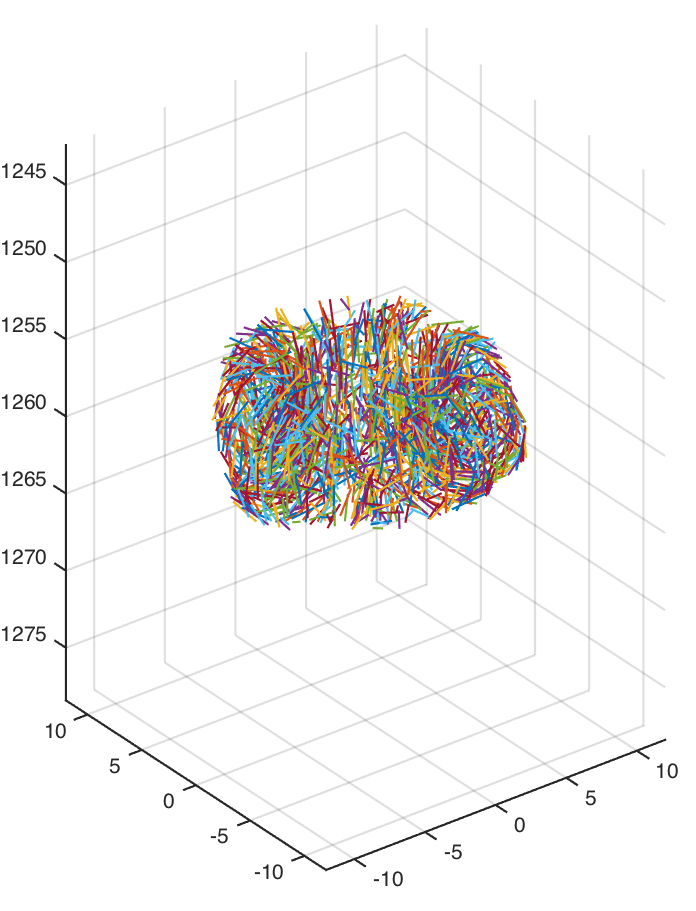
\includegraphics[width=\textwidth]{img/state_00250.pdf}
    \caption{$t=300$}\label{fig:sphere_simulation_1b}
  \end{subfigure}
  \begin{subfigure}[h]{0.4\textwidth}
    \centering
    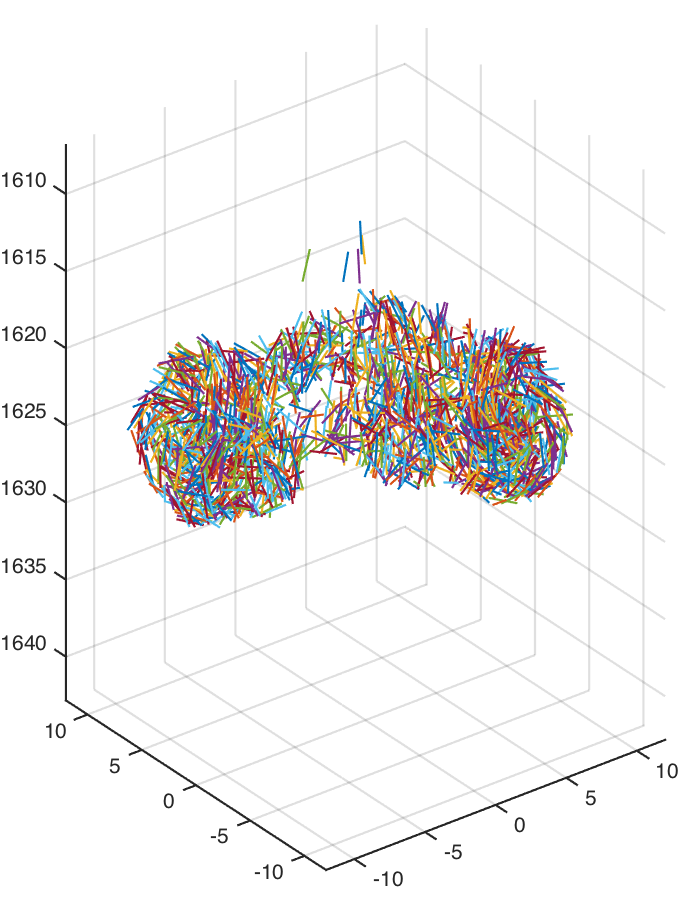
\includegraphics[width=\textwidth]{img/state_00350.pdf}
    \caption{$t=350$}\label{fig:sphere_simulation_1c}
  \end{subfigure}
  \begin{subfigure}[h]{0.4\textwidth}
    \centering
    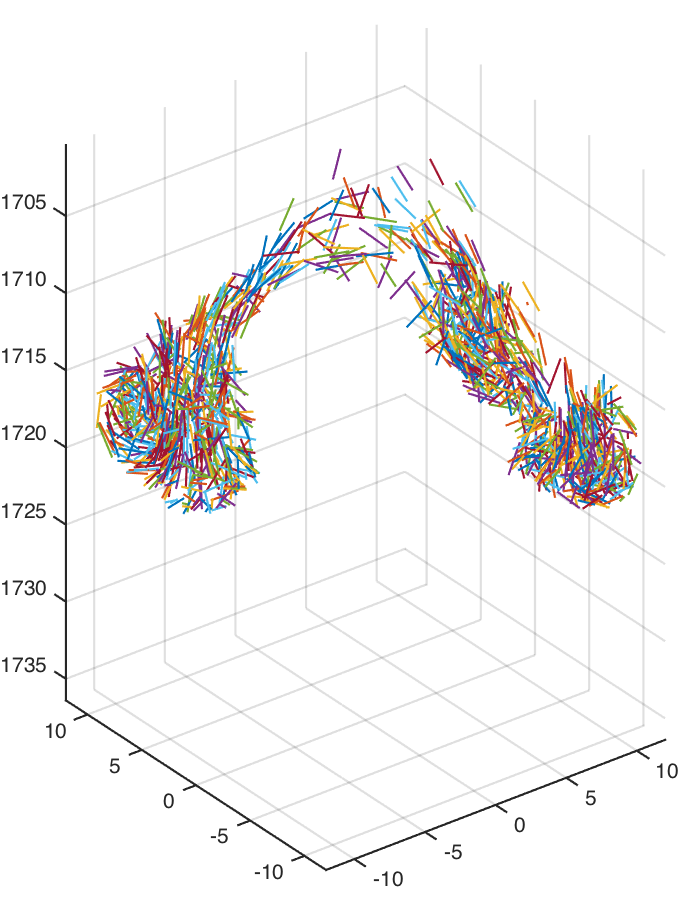
\includegraphics[width=\textwidth]{img/state_00380.pdf}
    \caption{$t=380$}\label{fig:sphere_simulation_1d}
  \end{subfigure}
  \caption[Visualization of sedimenting sphere.]{Visualization of sedimenting sphere. Fibers are randomly distributed inside a sphere and sediment due to gravity. The fibers proceed to form a turning torus. Eventually the torus breaks up into subclusters.}
  \label{fig:sphere_simulation}
\end{figure}

In Fig.~\ref{fig:sphere_simulation} we can see how the interacting fibers, beginning from the spherical shape, slowly start to form a continuously turning torus. Even though the behavior is more chaotic due to the large number of fibers and the random initial setup, this turning torus somewhat resembles the result for the tumbling orbits in Sec.~\ref{sec:example_ring}.

After some time the torus breaks and the fibers are split into multiple smaller cloudlets, which continue to sediment separately and slowly form their own smaller torus. However, due to tiny variations these toruses can be harder to see. 

The simulation of the presented example only takes $\~8$ seconds per timestep using the GPU implementation. Consequently it is possible to perform the $500$ time steps of the simulation in a little bit over $1$ hour. Simulating this many fibers in such a short time will allow for new research of this interesting phenomenon. One interesting question is to determine what influences the stability of the torus that is, when time does the torus break up.

\subsection{Sphere break-up}
\label{subsec:sphere_break}
To begin investigating this question we first define the stability of the torus in terms of the break up time. How to determine the exact break up time of the torus is quite challenging. This problem was also examined by Park et al.~\cite{Park2010}. In~\cite{Park2010} the break-up time is defined as the moment when the torus starts to bend prior to actually breaking. Unfortunately, they do not define a metric that determines the exact break up time. Based on the work in ~\cite{Park2010} we have developed a new measure of the break-up time.

We use the same definition for the torus as described by Park et al.~\cite{Park2010}. First we compute the initial horizontal radius $R_0$ of the sphere. As the cloud sediments and starts forming the torus, there is a small leakage fibers in its vertical tail. To find these fibers, such that they can be excluded from the active set of fibers defining the torus, we exclude all fibers with a distance larger than $R_0$ in the direction of gravity from the center of mass of the torus. For the remaining fibers we can compute the radius $R$ of the torus in each horizontal direction and the mean sedimentation velocity $V_z$. The torus metrics are illustrated for a sample run with $2000$ fibers and an average distance of $0.4$ in Fig.~\ref{fig:torus}. The horizontal radii $R_x$ and $R_y$ of the torus and the percentage of fibers remaining in the torus are shown in Fig.~\ref{fig:torus_radius} and Fig.~\ref{fig:torus_fibers}. The curves show the expected loss of fibers and the increasing torus radius.

\begin{figure}[!htbp]
  \centering
  \begin{subfigure}[h]{.48\textwidth}
	  \begin{tikzpicture}
	    \begin{axis}[
	      xlabel={Timestep},
	      ylabel={Radius},
	      width={\textwidth},
	      unbounded coords=discard,
	      xmin=0,xmax=500,
	      grid=major,
	      every axis label/.append style={font=\sffamily\footnotesize},
	      ]
	
	      \addplot[color=set11, very thick] table[x=Timestep,y=RadiusX,col sep=comma] {charts/sphere_2000_0040.csv};
	      \addplot[color=set12, very thick] table[x=Timestep,y=RadiusY,col sep=comma] {charts/sphere_2000_0040.csv};
	    \end{axis}
	  \end{tikzpicture}
    \caption{Torus horizontal radius.}\label{fig:torus_radius}
  \end{subfigure}
  \begin{subfigure}[h]{.48\textwidth}
	  \begin{tikzpicture}
	    \begin{axis}[
	      xlabel={Timestep},
	      ylabel={Fibers in torus (\%)},
	      width={\textwidth},
	      unbounded coords=discard,
	      xmin=0,xmax=500,
	      ymin=0.9,ymax=1.0,
	      grid=major,
	      legend pos=north east,
	      every axis label/.append style={font=\sffamily\footnotesize},
	      ]
	
	      \addplot[color=set11, very thick] table[x=Timestep,y=NormalizedN,col sep=comma] {charts/sphere_2000_0040.csv};
	
	    \end{axis}
	  \end{tikzpicture}
    \caption{Percentage of remaining fibers.}\label{fig:torus_fibers}
  \end{subfigure}
  \begin{subfigure}[h]{.48\textwidth}
	  \begin{tikzpicture}
	    \begin{axis}[
	      xlabel={Timestep},
	      ylabel={Radius},
	      width={\textwidth},
	      unbounded coords=discard,
	      xmin=0,xmax=500,
	      grid=major,
	      every axis label/.append style={font=\sffamily\footnotesize},
	      ]
	
	      \addplot[color=set12, mark=*,mark options={fill=white}, very thick] table[x=Timestep,y=RadiusZStd,col sep=comma] {charts/sphere_2000_0040_highlight.csv}
	node[pos=444, pin={[pin edge={color=set12, very thick}]min}]{};
	\addlegendentry{}
	      \addplot[color=set11, very thick] table[x=Timestep,y=RadiusZStd,col sep=comma] {charts/sphere_2000_0040.csv};
	    \end{axis}
	  \end{tikzpicture}
    \caption{Torus $\text{Radius}_z$ Standard Deviation.}\label{fig:torus_deviation}
  \end{subfigure}
  \begin{subfigure}[h]{.48\textwidth}
	  \begin{tikzpicture}
	    \begin{axis}[
	      xlabel={timestep},
	      ylabel={fibers in torus},
	      width={\textwidth},
	      unbounded coords=discard,
	      xmin=0,xmax=500,
	      grid=major,
	      legend pos=north east,
	      every axis label/.append style={font=\sffamily\footnotesize},
	      ]
	
	      \addplot[color=set11, very thick] table[x=Timestep,y=VelocityZ,col sep=comma] {charts/sphere_2000_0040.csv};
	
	      \legend{$V_z$}
	
	    \end{axis}
	  \end{tikzpicture}
    \caption{Mean sedimentation velocity.}\label{fig:torus_velocity}
  \end{subfigure}
  \caption[Evolution of the sedimenting torus.]{Evolution of the sedimenting torus. In the beginning the torus loses some fibers and the horizontal radii $R_x$ and $R_y$ increase slowly. The vertical radius $R_z$ undergoes a periodical contraction and expansion, which can also be seen in the peridocal change in the sedimentation velocity $V_z$. The eventual moment of the break-up of the torus is defined as the minimum standard deviation of the vertical radius $R_z^{\text{std}}$.}
  \label{fig:torus}
\end{figure}

In Fig.~\ref{fig:torus_deviation} we present the standard deviation of the radius in the direction of gravity as a function of time. We observe that the standard deviation of the radius in the direction of gravity for all fibers in the torus continuously decreases until it reaches a minimum value after which it starts to increase again. The time when the standard deviation reaches the minimum value can be identified visually to a few moments before the torus breaks up. We verified this metric manually against many simulations and it showed a great agreement with the visual moment of break-up. Using this metric we are now able to investigate the effect of the number and concentration of fibers on the stability and break up time of the torus.

A surprising insight was that the standard deviation of the radius $R_z$ seems to oscillate in Fig.~\ref{fig:torus_deviation}. This oscillation in the direction of gravity means that the torus is periodically expanding and shrinking until it breaks up. The same effect can also be seen in the mean sedimentation velocity $V_z$ of the torus in Fig.~\ref{fig:torus_velocity}. Since the periodical change in velocity is similar to the motion observed in the simple tumbling orbits experiment in Sec.~\ref{sec:example_ring},  this result strongly supports the idea that the turning torus with $2000$ fibers resembles a more chaotic version of the simplified tumbling orbits.

\subsection{Fiber concentration effect on break-up time}
\label{subsec:effect_concentration}

The first parameter to explore is the concentration of fibers, which we measure in terms of the average distance between a fiber and its closest neighbor. In the numerical experiments, we fixed the number of fibers at $2000$ and varied the concentration in the spherical cloud by varying its initial radius. The break-up time is estimated using the metric defined in Sec.~\ref{subsec:sphere_break}.

In Fig.~\ref{fig:concentration_breakup} the break-up time is presented as a function of the average distance between the fibers. We can see that there is a clear correlation. When the average distance between the fibers increases, i.e. a decrease in concentration, the time until the torus breaks up increases. When the cloud sediments and starts forming a torus, a large rotating velocity field is created in the fluid. The strength of this field depends on how strong the interaction between the fibers is. When the fibers are far apart the interaction between the fibers is small and the rotating motion will not be as strong, leading to a longer break-up time.

\begin{figure}[!htbp]
  \centering
  \begin{tikzpicture}
    \begin{axis}[
      xlabel={Average distance},
      ylabel={Break-up time step},
      width={0.618033989\textwidth},
      unbounded coords=discard,
      xmin=0,xmax=3,
      ymin=0,ymax=1800,
      grid=major,
      ]

      \addplot[color=set11, mark=*,mark options={fill=white}, very thick] table[x=Concentration,y=Break] {charts/concentration_breakup.csv};

    \end{axis}
  \end{tikzpicture}
  \caption[Effect of fiber concentration on torus break up time.]{Effect of fiber concentration on torus break up time. Given a fixed number of fibers, if the average distance between fibers is very low, i.e. the fiber concentration is very high, than the break-up occurs earlier. If the average distance is high the break-up takes longer.}
  \label{fig:concentration_breakup}
\end{figure}

\subsection{Number of fibers effect on break up time}
\label{subsec:effect_number}

The second parameter we studied was the number of fibers. In this set of experiments, the concentration is fixed by keeping the average distance between the fibers fixed to $0.4$. We measure the break up time as we vary the number of fibers from $100$ to $2000$. In Fig.~\ref{fig:number_breakup} the result is displayed. Here we find that there is a positive correlation between the number of fibers and the break-up time, however not as strong as in the case when we varied the concentration in Sec.~\ref{subsec:effect_concentration}. These results match the results found by Park et al.~\cite{Park2010}.

The results presented in Sec.~\ref{} and Sec.~\ref{} show that both fiber concentration and the number of fibers affect the break-up time of the torus. Future research should explore these correlations closer and include other studies such as the dependence of the initial shape of the cloud on the process.

\begin{figure}[!htbp]
  \centering
  \begin{tikzpicture}
    \begin{axis}[
      xlabel={Number of fibers},
      ylabel={Break-up time step},
      width={0.618033989\textwidth},
      unbounded coords=discard,
      xmin=0,xmax=2000,
      ymin=0,ymax=1800,
      grid=major,
      ]
      \addplot[color=set11, mark=*,mark options={fill=white}, very thick] table[x=M,y=Break] {charts/number_breakup.csv};

    \end{axis}
  \end{tikzpicture}
  \caption[Effect of number of fibers on torus break up time.]{Effect of number of fibers on torus break up time. Given a constant fiber concentration, if the number of fibers is small than the break-up occurs earlier. If the number of fibers is large the break-up takes longer.}
  \caption{Effect of number of fibers on torus break up time.}
  \label{fig:number_breakup}
\end{figure}

These two results show that both the concentration and the number of fibers have an effect on the break up time of the torus. Future research should explore these correlations closer as our tests only looked at two parameters in isolation. How other parameters, like external forces, the numerical accuracy and the initial fiber distribution affect the stability of the torus are promising questions.

\section{Mixed density sphere}
\label{sec:mixed_density_sphere}

The final experiment we performed resembles the setup investigated by Bülow et al.~\cite{Bulow2015}. In this setup instead of identical fibers, we look at the mixing of fibers with different densities. We divide the total number of fibers into two different density groups and arrange them inside a sphere, which again sediments due to gravity. To separate the two groups visually, they are colored in red and blue. The blue group has the lower density and the red group the higher density. The ratio between the densities is set to $\text{blue} / \text{red}= 0.75 / 1.0$.

Fig.~\ref{fig:unmixed_sphere} shows different timesteps of a simulation where the two density groups are separated into the top and bottom half of the sphere. Since the fibers are clearly separated, this particular configuration is referred to as an unmixed sphere. The higher density group is on top and the lower density group is at the bottom (Fig.~\ref{fig:mixing_top_a}). After a few timesteps the higher density fibers have almost completely dropped through the lower density fibers (Fig.~\ref{fig:mixing_top_b}). The falling high density fibers cause a large number of low density fibers to be ejected from the sphere. Both groups then proceed to almost independently form the characteristic torus observed in the previous experiment in Sec.~\ref{sec:example_sphere} (Fig.~\ref{fig:mixing_top_c}). The higher density fibers, however, form a larger torus with a lower fiber concentration. This lower concentration also causes them to lose velocity, which in turn allows the lower density fibers to drop through the larger outer torus (Fig.~\ref{fig:mixing_top_d}). Both toruses are not very stable and soon afterwards break apart.

\begin{figure}[!htbp]
  \centering
  \begin{subfigure}[h]{0.24\textwidth}
    \centering
    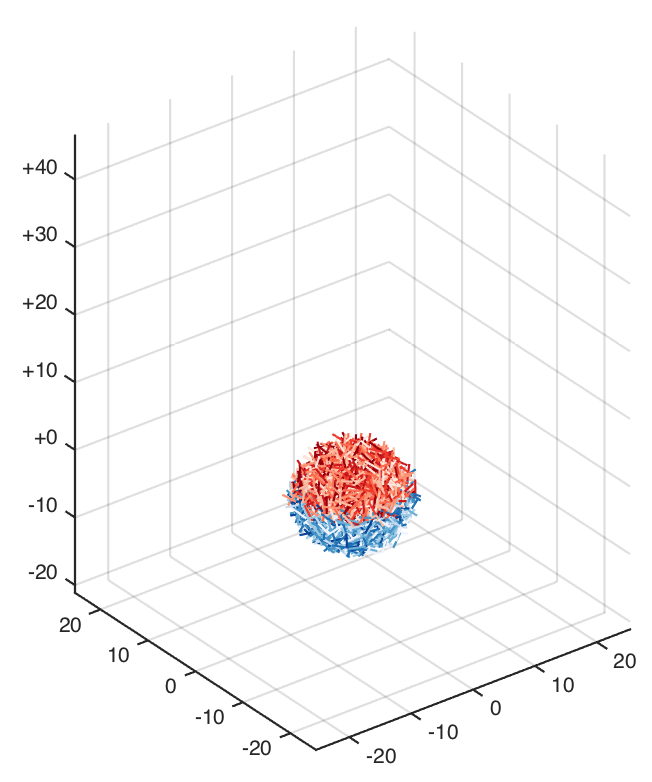
\includegraphics[width=\textwidth]{img/mixing/top_00000.pdf}
    \caption{$t=0$}\label{fig:mixing_top_a}
  \end{subfigure}
  \begin{subfigure}[h]{0.24\textwidth}
    \centering
    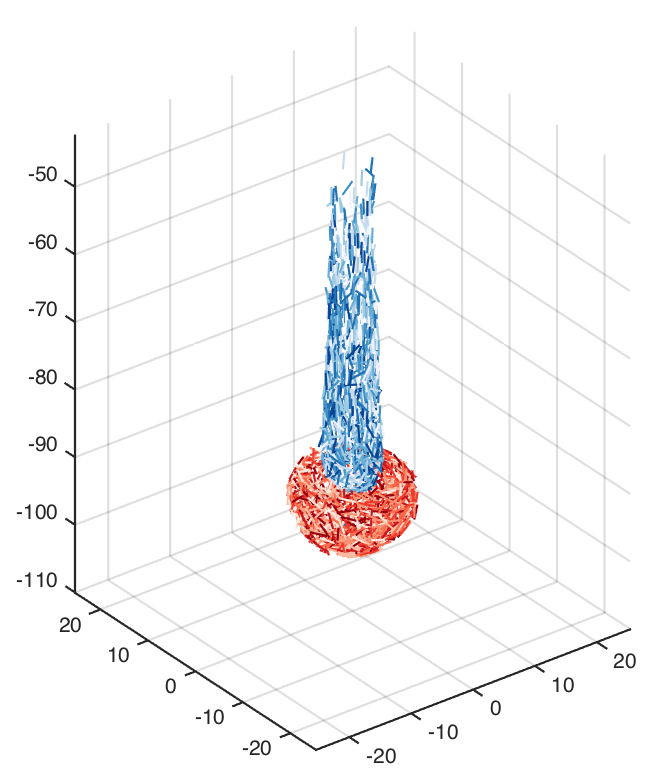
\includegraphics[width=\textwidth]{img/mixing/top_00020.pdf}
    \caption{$t=20$}\label{fig:mixing_top_b}
  \end{subfigure}
  \begin{subfigure}[h]{0.24\textwidth}
    \centering
    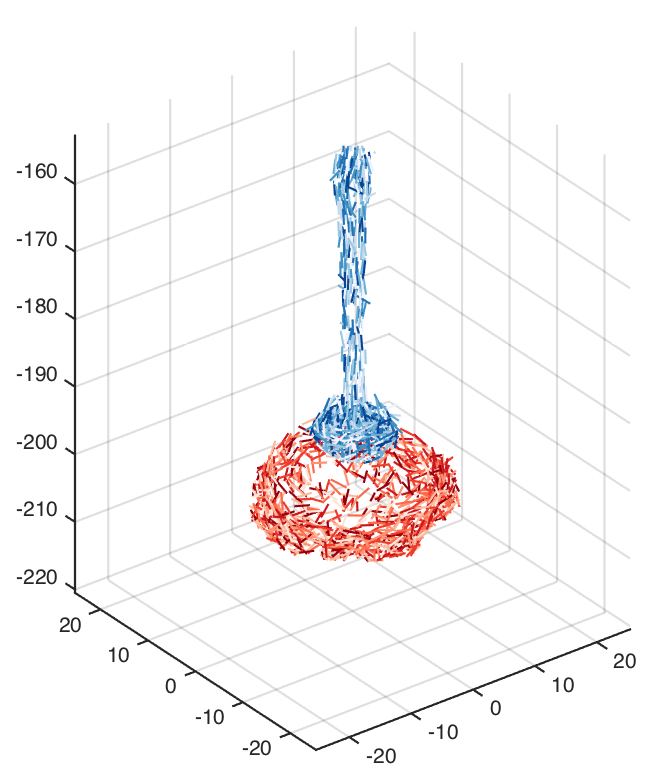
\includegraphics[width=\textwidth]{img/mixing/top_00060.pdf}
    \caption{$t=60$}\label{fig:mixing_top_c}
  \end{subfigure}
  \begin{subfigure}[h]{0.24\textwidth}
    \centering
    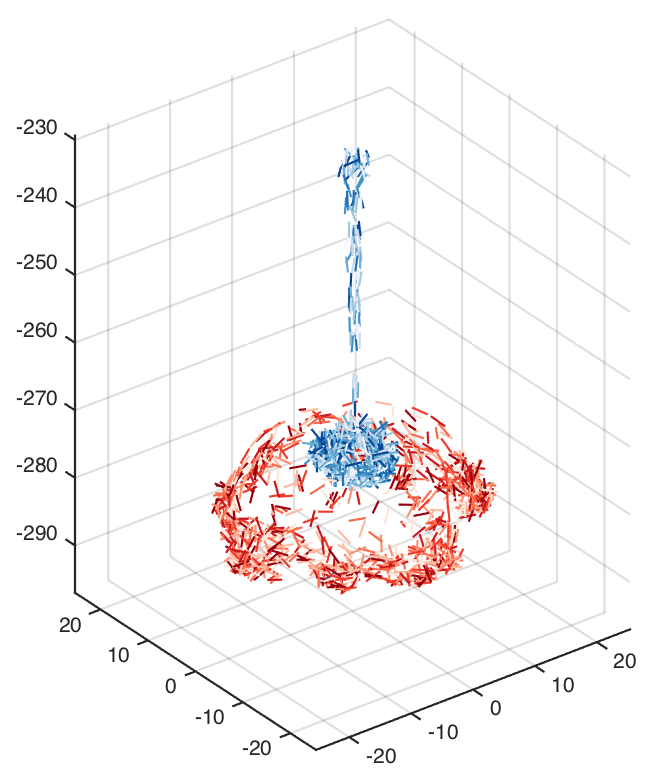
\includegraphics[width=\textwidth]{img/mixing/top_00100.pdf}
    \caption{$t=100$}\label{fig:mixing_top_d}
  \end{subfigure}
  \caption[Unmixed sphere]{Unmixed sphere. Starting the sedimentation with the high density fibers (red) as the top half and the low density fibers (blue) as the bottom half of the sphere.}
  \label{fig:unmixed_sphere}
\end{figure}

In contrast to the configuration with an unmixed sphere, Fig.~\ref{fig:mixed_sphere} shows a similar simulation, starting with a randomly mixed sphere (Fig.~\ref{fig:mixing_random_a}). The beginning of the simulation behaves similar to the unmixed case, but the separation does not happen as fast and far fewer lower density fibers are lost from the sphere (Fig.~\ref{fig:mixing_random_b}). Both the larger higher density and the smaller lower density torus form again. Yet in contrast to the unmixed case both groups stay closer together. The close proximity prevents the groups from completely separating and causes the higher density torus to be sucked down by the passing lower density torus (Fig.~\ref{fig:mixing_random_c}). During the following timesteps the two toruses appear to form an interlocked torus, which continues to sediment  (Fig.~\ref{fig:mixing_random_d}). Eventually the interlocked torus breaks up and fibers scatter. 

\begin{figure}[!htbp]
  \centering
  \begin{subfigure}[h]{0.24\textwidth}
    \centering
    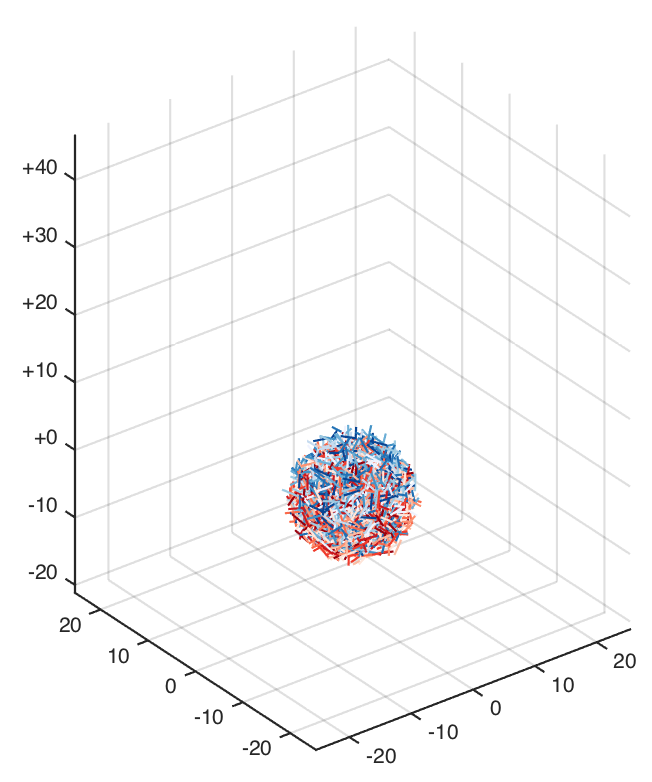
\includegraphics[width=\textwidth]{img/mixing/random_00000.pdf}
    \caption{$t=0$}\label{fig:mixing_random_a}
  \end{subfigure}
  \begin{subfigure}[h]{0.24\textwidth}
    \centering
    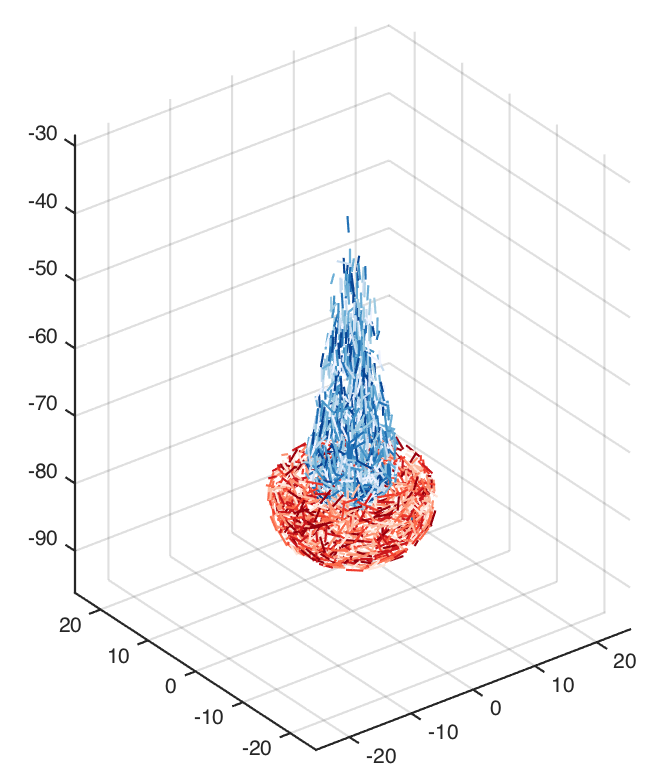
\includegraphics[width=\textwidth]{img/mixing/random_00020.pdf}
    \caption{$t=20$}\label{fig:mixing_random_b}
  \end{subfigure}
  \begin{subfigure}[h]{0.24\textwidth}
    \centering
    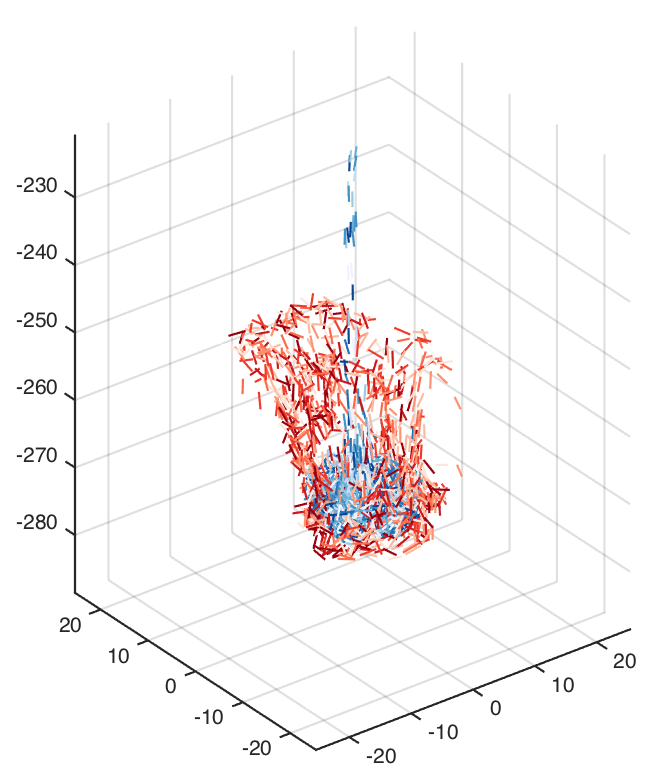
\includegraphics[width=\textwidth]{img/mixing/random_00100.pdf}
    \caption{$t=100$}\label{fig:mixing_random_c}
  \end{subfigure}
  \begin{subfigure}[h]{0.24\textwidth}
    \centering
    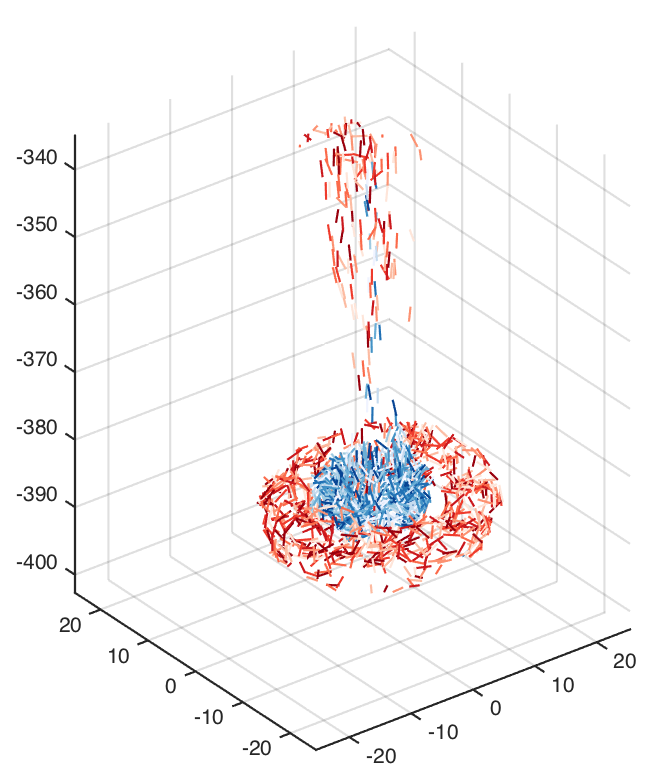
\includegraphics[width=\textwidth]{img/mixing/random_00150.pdf}
    \caption{$t=150$}\label{fig:mixing_random_d}
  \end{subfigure}
  \caption[Mixed sphere]{Mixed sphere. Starting the sedimentation with the high density fibers (red) and the low density fibers (blue) randomly mixed inside the sphere.}
  \label{fig:mixed_sphere}
\end{figure}

The results for the mixed and unmixed sphere with rigid straight fibers do largely agree with the results of spherical particles from Bülow et al.~\cite{Bulow2015}. However, both simulation methods and setups are very different which makes a comparison very challenging. Furthermore our experiment are only a first step and many more experiments have to be cared out to get a deeper understanding of the behavior of rigid fibers in a mixed sphere. Exploring the impact of initial fiber configuration, the density ratio and the fiber concentration are all exciting future research opportunities.


\chapter{Conclusion}

In this thesis we have developed a completely new parallel GPU implementation for the numerical simulation of rigid fibers suspension using CUDA. This is faster and therefore many more fibers can be simulated than before. Furthermore being able to simulate more fibers enables the researcher to perform more extensive and in-depth studies of the various properties of the flow and simulation.

Based on the theoretical foundation of the simulated model and the original serial Fortran implementation we rewrote the algorithm to take advantage of massively parallel computational power available in modern GPUs. We outlined the required steps to implement the algorithm using CUDA. We investigated a number of different optimizations to further improve the performance. These explored optimizations included variations of the algorithm, GPU specific implementation details and the choice of linear solver. To reach the goal of comparing the performance between CPU and GPU the new parallel algorithm was backported to the CPU using OpenMP. Thereby improving the fairness of the comparison as much as possible.

During extensive benchmarking we showed that variations perform differently depending on the underlying architecture. Optimizations developed for the CPU implementation actually slow down the GPU implementation due to diverging execution branches. We also discovered that off-the-shelf GPU implementations of iterative solvers can be slower compared to their highly optimized CPU alternatives. Hopefully future research in this area will allow for even better performance of iterative solvers on the GPU.

Overall our GPU simulation on the NVIDIA GTX 970 is able to outperform the CPU version on an Intel Core i7 4770 by a factor of $20×$ to $40×$. This allows the GPU simulation to handle up to $2000$ fibers, which is more than double then before, and only takes $8$ seconds to advance one time step on a desktop computer.

To test and validate our new parallel implementation, we performed a number of simulations of known experiments for sedimenting fibers. Using the test-case of tumbling orbits we showed that the numerical precision of our single precision implementation is able to reproduce the result obtained from the former double precision Fortran simulations. We also explored how the performance of iterative solvers is affected by the fiber concentration, showing that if fibers come too close the number of iterations increases and slows down the simulation. Our last experiment looked at the known phenomena that a sphere of fibers sedimenting form a torus and eventually break up into smaller clusters. Our results show an excellent agreement with both experimental and numerical work performed previously. Additionally, we showed that the stability of the torus is positively correlated with the increasing distance between fibers and the total number of fibers. Further research in this area is helped greatly by the fact that new case can rapidly be explored using our fast GPU simulation.

Currently the number of fibers in our simulation is limited by the amount of memory available on the GPU. In future we would like to research how to lift this restriction. One possible research direction is to avoid storing the matrix completely. Instead the required computation would have to be carried out iteratively and on-demand. This would allow for a practical unlimited number of fibers with the cost of an largely increased computation time. If this trade off is worth it remains to be seen.
Figure
Another exciting possibility is the move to a multi-device setup. Using multiple GPUs simultaneously would enable much larger systems, if the workload can be split efficiently. MAGMA, the library used for the GPU direct solver, offers a couple of interesting options in this area. The most challenging part to efficient parallelization is solving the system and broadcasting the result across multiple device. The other steps of the algorithm can be naturally partitioned and have already been implemented across multiple CPUs using OpenMPI.

Finally, to further improve the simulation it might be worth looking at the numerical algorithm itself. Adapting a different algorithm based on the fast summation method might not only improve the performance but also reduce the required memory allowing for faster and larger simulation. How this affects the accuracy and behavior of the simulation is an interesting future research question.


\printbibliography
\clearpage

\appendix
\addappheadtotoc
\begin{table}[!htbp]
  \caption*{Parameters for tumbling orbits experiment in Sec~\ref{sec:example_ring}.}
  \begin{center}
    \begin{tabulary}{\textwidth}{LR}
      \toprule
      Parameter & Value \\
      \midrule
      Number of fibers & $16$ \\
      Concentration & $0.2146$ \\
      Timestep & $0.1$ \\
      Slenderness & $0.01$ \\
      Number of terms in force expansion & $5$ \\
      Number of quadrature intervals & $8$ \\
      Number of quadrature points per interval & $3$ \\
      \bottomrule
    \end{tabulary}
  \end{center}
\end{table}

\begin{table}[!htbp]
  \caption*{Parameters for GMRES iterations experiment in Sec~\ref{sec:example_concentration_gmres}.}
  \begin{center}
    \begin{tabulary}{\textwidth}{LR}
      \toprule
      Parameter & Value \\
      \midrule
      Number of fibers & $2000$ \\
      Concentration & $0.02–40.96$ \\
      Timestep & $0.1$ \\
      Slenderness & $0.01$ \\
      Number of terms in force expansion & $5$ \\
      Number of quadrature intervals & $8$ \\
      Number of quadrature points per interval & $3$ \\
      \bottomrule
    \end{tabulary}
  \end{center}
\end{table}

\begin{table}[!htbp]
  \caption*{Parameters for sedimenting sphere experiment in Sec~\ref{sec:example_sphere}.}
  \begin{center}
    \begin{tabulary}{\textwidth}{LR}
      \toprule
      Parameter & Value \\
      \midrule
      Number of fibers & $2000$ \\
      Concentration & $0.2$ \\
      Timestep & $0.1$ \\
      Slenderness & $0.01$ \\
      Number of terms in force expansion & $5$ \\
      Number of quadrature intervals & $8$ \\
      Number of quadrature points per interval & $3$ \\
      \bottomrule
    \end{tabulary}
  \end{center}
\end{table}

\begin{table}[!htbp]
  \caption*{Parameters for fiber concentration effect on break-up in Sec~\ref{subsec:effect_concentration}.}
  \begin{center}
    \begin{tabulary}{\textwidth}{LR}
      \toprule
      Parameter & Value \\
      \midrule
      Number of fibers & $2000$ \\
      Concentration & $0.08–2.56$ \\
      Timestep & $0.1$ \\
      Slenderness & $0.01$ \\
      Number of terms in force expansion & $5$ \\
      Number of quadrature intervals & $8$ \\
      Number of quadrature points per interval & $3$ \\
      \bottomrule
    \end{tabulary}
  \end{center}
\end{table}

\begin{table}[!htbp]
  \caption*{Parameters for number of fibers effect on break-up in Sec~\ref{subsec:effect_number}.}
  \begin{center}
    \begin{tabulary}{\textwidth}{LR}
      \toprule
      Parameter & Value \\
      \midrule
      Number of fibers & $100–2000$ \\
      Concentration & $0.4$ \\
      Timestep & $0.1$ \\
      Slenderness & $0.01$ \\
      Number of terms in force expansion & $5$ \\
      Number of quadrature intervals & $8$ \\
      Number of quadrature points per interval & $3$ \\
      \bottomrule
    \end{tabulary}
  \end{center}
\end{table}

\begin{table}[!htbp]
  \caption*{Parameters for un/mixed sphere in Sec~\ref{sec:mixed_density_sphere}.}
  \begin{center}
    \begin{tabulary}{\textwidth}{LR}
      \toprule
      Parameter & Value \\
      \midrule
      Number of fibers & $2000$ \\
      Concentration & $0.4$ \\
      Timestep & $0.1$ \\
      Slenderness & $0.01$ \\
      Number of terms in force expansion & $5$ \\
      Number of quadrature intervals & $8$ \\
      Number of quadrature points per interval & $3$ \\
      \bottomrule
    \end{tabulary}
  \end{center}
\end{table}


\end{document}
